
% Background Chapter
%%%
% New organisation:
%
% Introduction and Literature Review
%   Tropospheric ozone and air quality . . . . .
%   Isoprene and other VOCs . . . . . . . . . . .
%   Formaldehyde (HCHO) . . . . . . . . . . . .
%   Models . . . . . . . . . . . . . . . . . . . . .
%   Aims?
%%%%%%
\chapter{Introduction and Literature Review} % Chapter Title
\label{LR}

\section{Tropospheric ozone and air quality}
  \label{LR:O3andAQ}
  \subsection{Air Quality}
    \label{LR:O3andAQ:AQ}
    %%% AUSTRALIA
    Australia is largely covered by environments which are not heavily influenced by human activity.
    These regions are natural (biogenic) sources of the trace gases (those which make up less than 1\% of the earth's atmosphere).
    Trace gases in the atmosphere can have a large impact on living conditions.
    They react in complex ways with other elements (anthropogenic and natural), affecting various ecosystems upon which life depends.
    Biogenic emissions affect surface pollution levels, potentially enhancing particulate matter (PM) and ozone levels.
    
    \subsubsection{Ozone}
      %%% OZONE
      Ozone (O$_3$) is mostly located in the stratosphere, where it helpfully prevents much of the shorter wave length solar radiation from reaching the earth's surface (ie UV light).
      However around 11\% of the total column of ozone is located in the troposphere (TODO: cite), where it has several deleterious effects.
      Ozone in the lower atmosphere is a serious hazard that causes health problems \citep{Hsieh2013}, damages agricultural crops worth billions of dollars \citep{Avnery2011,Yue2017}, and increases the rate of climate warming \citep{IPCC_2013_chap8}.
      Around 5 to 20 percent of all air pollution related deaths are due to ozone (\cite{Monks2015}).
      In the short term, ozone concentrations of $\sim$50-60~ppbv over eight hours or $\sim$80~ppbv over one hour are agreed to constitude a human health hazard \citep{Ayers2006,Lelieveld2009}. 
      Long term exposure to lower levels cause problems with crop loss and ecosystem damage \citep{Emberson2003}, and both short and long term concentrations may get worse in the future \citep{Lelieveld2009, Stevenson2013}.
      Further tropospheric ozone enhancements are projected to drive reductions in global crop yields equivalent to losses of up to \$USD$_{2000}$ 35 billion per year by 2030 \citep{Avnery2011}, along with detrimental health outcomes equivalent to $\sim$\$USD$_{2000}$11.8 billion per year by 2050 \citep{Selin2009}.
      Recently \cite{Yue2017} showed that the net effect of near-surface ozone on is a $\sim 14\%$ decrease in net primary productivity (NPP) in China, which could be reduced with drastic measures required to reduce this by $70\%$ by 2030.
      
      The tropospheric ozone concentrations rely on climate and ozone precursor emissions; including NO, NO$_2$, CO, VOCs, and HCHO \citep{Atkinson2000, Young2013, Marvin2017}. 
      Ozone predictions are uncertain and difficult due to the vagaries of changing climate which affects both transport, deposition, destruction, and plant based precursor emissions.
      All of these processes are tightly coupled and difficult to accurately model, as they depend on uncertain assumptions such as CO$_2$ dependency \citep{Young2013}.
      Even with all the work done in the prior decades there remains large uncertainties about ozone precursors in the troposphere \citep{Mazzuca2016}.
      Ozone is also a very important substance for formation of radicals (NO$_3$, OH) in the troposphere through photolysis in the presence of water.
    
    \subsubsection{Particulate matter and SOA}
      %%% PM and SOA
      PM in the atmosphere is also a major problem, causing an estimated 2-3 million deaths annually \citep{Hoek2013, Krewski2009, Silva2013, Lelieveld2015}. 
      Aerosols are suspended particulates and liquid compounds in the atmosphere, of which particulate matter (PM) is an important subset.
      Fine particulate matter (PM$_{2.5}$) penetrates deep into the lungs and is detrimental to human health.
      Some PM comes from small organic aerosols (OA) emitted in the particulate phase and referred to as primary OA (POA).
      A substantial amount of PM is due to gaseous organic compounds transforming in the troposphere leading to what's known as secondary OA (SOA) \citep{Kroll2008}.
      Formation of SOA is generally due to VOC oxidation and subsequent reactions, while removal from the atmosphere is largely due to wet or dry deposition, and cloud scavenging \citep{Kanakidou2005}.
    
    
    \subsubsection{Factors influencing ozone and PM}
      %\label{LR:O3andAQ:AQfactors}
      
      %%% Important factors affecting PM and Ozone
      One important factor, affecting both PM and ozone concentration, is a group called Volatile Organic Compounds (VOCs).
      The major source of VOCs in the atmosphere is biogenic, with around 90\% of emissions (globally) coming from natural sources \citep{Guenther1995,Guenther2006, Millet2006}.
      Global non-methane VOC (NMVOC) levels are estimated at 85~\%, 13~\%, and 3~\% from biogenic, anthropogenic, and pyrogenic sources respectively \citep{Kefauver2014}.
      They also and affect radical levels, which drive much of the chemistry in our atmosphere.
      Methane and isoprene each comprise around a third of the global total emissions of VOCs (\cite{Guenther2006}).
      However, methane is relatively long lived (years) and is well mixed in the atmosphere while isoprene levels are very volatile and spatially diverse due to a life time of around an hour.
      This means that methane measurements and concentrations are relatively well understood, while NMVOCs are less so.
      
      Due to the lack of in-situ ground based measurements, estimates of VOC emissions are uncertain, with large scale extrapolation required \cite{Millet2006}.
      VOC emission estimates are based on (and highly sensitive to) many factors, including plant type and soil moisture \citep{Guenther1995}, neither of which are well characterised in Australia \citep{Sindelarova2014, Bauwens2016}.
      Changes in parameterisation of soil moisture in the Model of Emissions of Gases and Aerosols from Nature (MEGAN, \cite{Guenther1995}) lead to massive changes in Australian isoprene emission estimates \citep{Sindelarova2014}.
      This has an compounding effect on the large uncertainties of biogenic VOC emissions \citep{Guenther2000, Millet2006}.
      
      Another important factor is NO$_X$ (NO, NO$_2$) which has a complex non-linear relationship with both ozone and VOCs.
      The role of NO$_X$ on VOC oxidation is discussed in more detail in Section \ref{LR:VOCs:IsopCascade}.
      Since many Australian cities are on the edge of regions with rich VOC emissions, it is very important to clarify the quantity, type, and cause of VOC emissions.
      The existence of satellite data covering remote areas provides an opportunity to improve VOC emissions estimates leading to more robust models of global climate and chemistry.
      Understanding of emissions from these areas is necessary to inform national policy on air pollution levels.
      
      %%% FIRE smoke plumes
      Smoke plumes from biomass burning can carry ozone precursors, creating higher ozone concentrations downwind of the plume's source.
      Fire emissions include a range of chemicals and each year the affects of fire or burning seasons blanket the northern and southern hemispheres independently.
      Biomass burning in southern Africa and South America has previously been shown to have a major influence on atmospheric composition in Australia \citep{Oltmans2001, Gloudemans2006, Edwards2006}, particularly from July to December \citep{Pak2003, Liu2016}.
    
    \subsubsection{How do we measure air quality?}
    
      % Air Quality metric example
      Australian air quality is monitored independently within each state, using various metrics. These metrics are measured by varying numbers of monitoring stations in each state.
      In New South Wales (NSW) the metrics used to determine air quality are: particulate matter (PM), O$_3$, CO, NO$_2$, SO$_2$, and visibility.
      PM is separated into size bins: with radius $< 2.5 $~$\mu$m and $<10$~$\mu$m being PM$_{2.5}$, and PM$_{10}$ respectively.
      An air quality index equal to the worst of these metrics is used for NSW as shown at \url{http://www.environment.nsw.gov.au/aqms/aqitable.htm}.
      Similar methods are used in other states to get an idea of air quality.
      Measurement stations are generally located in population centres, and don't regularly measure precursor emissions. 
      This is an important omission as naturally emitted precursor gases often get transported into cities where they affect air quality.
      
      Australia is dominated by areas with little anthropogenic influence and no ground based measurements of the natural emissions taking place \citep{VanDerA2008}.
      One source of information which covers the entirety of Australia is remote sensing data.
      This comes from instruments on satellites which overpass daily recording reflected solar (and emitted terrestrial) radiation.
      In conjunction with atmospheric chemistry and radiative models, these measurements can be used to quantify the abundance of several chemical species in the atmosphere.
      These measurements can then be used to determine the unmeasured emissions of precursor gases which affect air quality.
      Satellite data allow us to verify large scale model estimates of natural emissions.
      Satellite measurements can be performed using spectral fitting followed by conversion to vertical column densities.
      The use of multiple satellites can even be used to detect intradiel concentrations in trace gas columns, as shown in \cite{Stavrakou2015} using OMI and GOME-2 measurements, which have respective overpass times of 1330 and 0930 LT.
      These various measurements can be used to improve models, which allows prediction of harmful and costly events, and prevention of scenarios in which pollution events are likely.
      
      In Australia most long term air quality measurements are performed in or near large cities.
      Estimates of atmospheric gas and particulate densities, and their distributions over much of the continent are uncertain, lacking long term in-situ measurements.
      Although the majority of VOC emissions globally are from biogenic sources, anthropogenic emissions in populated areas must be managed.
      \cite{Millet2008} show that anthropogenic emissions of HCHO in America are mostly negligible, although improved sensitivity from oversampling allowed satellite detection of enhanced HCHO concentrations over Houston and Texas \citep{Zhu2014}.
      This is not the case in China, since massive population centres and industrial districts are emitting huge amounts of VOCs into the atmosphere \citep{Fu2007}.
      \cite{Fu2007} use GOME measurements over Asia and derive biogenic, anthropogenic, and pyrogenic VOC emissions, and \cite{Zhu2014} use oversampling of the OMI HCHO measurements to determine anthropogenic highly-reactive VOC emissions.
      Then with their updated emissions they show how surface ozone is affected, with a seasonal increase of 5-20~ppb simulated by GEOS-Chem.
      
      Many models lack in-situ measurements with which to verify their chemical mechanisms, leading to large discrepancies, as seen in \cite{Marvin2017a}.
      TODO: briefly talk about Marvin2017a takeaways.
      
      In-situ measurements also contain errors, depending on the device used and chemical being measured this error can be significant.
      \cite{Dunne2017} analyse the uncertainty of VOC measurements (including isoprene) using three different techniques during a campaign in Sydney in 2012.
      The major sources of uncertainty in measurement techniques included interference from non-target compouds and under-reporting.
      Overall isoprene uncertainty in their dataset of isoprene measurements was a factor of 1.5 to 2.
      This can feed into uncertainties in modelling and satellite retrievals, as verification and correlations are affected.
      
      % Ozone sondes
      Since the Montreal Protocol on Substances that Deplete the Ozone Layer was established in August 1987, and ratified in August 1989, several satellites and many measurement stations were set up to monitor ozone in the stratosphere.
      However, in the southern hemisphere there are relatively few records of ozone (\cite{Huang2017}).
      One method of measuring ozone in the troposphere and stratosphere is by releasing weather balloons (with attached ozone detectors) which take readings as they rise up to around 30~km, giving a vertical profile of concentrations.
      Since 1986, Lauder, New Zealand (45$^{\circ}$S, 170$^{\circ}$E) has released ozonesondes allowing a multi-decadal analysis of ozone concentrations over the city \citep{Brinksma2002}.
      Kerguelan Island (49.2$^{\circ}$S, 70.1$^{\circ}$E), also has a record of ozonesonde profiles, which are directly in the path of biomass burning smoke plumes transported off shore from Africa \citep{Baray2012}.
      SHADOZ is the southern hemispheric additional ozone project, which have released sondes from 15 sites at different times \url{http://tropo.gsfc.nasa.gov/shadoz/}.
      
      
    %\subsubsection{Satellite measurements}
      % Satellite measurements
      TODO: get access to Hegglin (\url{10.1038/ngeo604}) \citep{Hegglin2009}
      TODO: Include ozone hole treaty and things put in place for that
      
      Combining satellite data with model outcomes provides a platform for the understanding of natural processes which is especially useful over Australia.
      Due to the low availability of in-situ data over most of the Australian continent, a combination of the models with satellite data may provide improved understanding of emissions from Australian landscapes.
      Improved emissions estimates will in turn improve the accuracy of CTMs, providing better predictions of atmospheric composition and its response to ongoing environmental change.
      
      Box models are much smaller scale than global CTMs, examining one uniform environment with many parametrisations such as transport and emissions.
      Box models can be used to check chemical mechanisms in specific scenarios, such as high or low NO$_X$ environments.
      \cite{Marvin2017} use a box model matching conditions in southeast USA to evaluate isoprene mechanisms from several models.
      
      %Satellite Errors
      While satellite data is effective at covering huge areas (the entire earth) it only exists at a particular time of day, is subject to cloud cover, and generally does not have fine horizontal or vertical resolution.
      Concentrations retrieved by satellites have large uncertainties, which arise in the process of transforming spectra to total column measurements, as well as instrument degradation (satellite instruments are hard to tinker with once they are launched).
      Uncertainty in transforming satellite spectra comes from a range of things, including measurement difficulties introduced by clouds, and instrument sensitivity to particular aerosols \citep{Millet2006}.
      Many products require analysis of cloud and aerosol properties in order to estimate concentration or total column amounts \citep{Palmer2001,Palmer2003, Marais2012, Vasilkov2017}.
      There are two types of error, arguably the worst of these is systematic error (or bias) which normally indicates a problem in calculation or instrumentation.
      If the systematic error is known, it can be corrected for by either offsetting data in the opposite direction, or else fixing the cause.
      A proper fix can only be performed if the sources of error are known and there is a way of correcting or bypassing it.
      Random error is the other type (often reported as some function of a datasets variance, or uncertainty), and this can be reduced through averaging either spatially or temporally. 
      By taking the average of several measurements, any random error can be reduced by a factor of one over the square root of the number of measurements.
      This is done frequently for satellite measurements of trace gases (which are often near to the detection limit over much of the globe).
      For example: \cite{Vigouroux2009} reduce the measurement uncertainty (in SCIAMACHY HCHO columns) by at least a factor of 4 through averaging daily over roughly 500km around Saint-Denis, and only using days with at least 20 good measurements.
      The main source of error in satellite retrievals of HCHO are due to instrument detection sensitivities, and the vertical multiplication factor (discussed in more detail in Section \ref{BioIsop:Uncertianty:Satellite}) \citep{Millet2006}.
      
  \subsection{Ozone transported from the stratosphere}
    
    What drives ozone in the troposphere? Two main contributors are transport from the stratosphere and creation due to biogenic emissions of precursors. 
    At smaller (regional) scales anthropogenic emissions are also important, especially in large cities such as Sydney due to NO$_X$ emissions from traffic and power production.
    
    In the stratosphere ozone production is generally driven by the Chapman mechanism, as high energy light (with wavelengths $\lambda<242$~nm) photolyses the molecular oxygen (O$_2$) in the atmosphere \citep[][Chapter 3, section 2]{BrasseurJacob2017}.
    The Chapman mechanism involves several equations which lead to rough equilibrium of O, O$_2$, O$_3$ and pressure, as follows:
    \begin{eqnarray*}
    	\label{LF:eqn:Chapman}
    	\textrm{O}_2 + hv(\lambda < 242 \text{nm}) & \rightarrow & \text{O} + \text{O} \\
    	\text{O} + \text{O}_2 + \text{M} & \rightarrow & \text{O}_3 + \text{M} \\
    	\text{O}_3 + hv(\lambda < 1180 \text{nm}) & \rightarrow & \text{O} + \text{O}_2 \\
    	\text{O} + \text{O}_3 & \rightarrow & \text{O}_2 + \text{O}_2 \\
    \end{eqnarray*}
    Where $hv$ represents radiation and M is an inert molecule (such as N$_2$).
    The high energy photons ($\lambda < 242$~nm) are present from the top of the atmosphere but are mostly removed before reaching the troposphere.
    The lifetime of O against loss by O$_2$ is less than a second in the troposphere, and produced O$_3$ quickly returns to O and O$_2$, as low energy ($\lambda < 1180$~nm) light and M are abundant.
    The gradient of light penetration in addition to the logarithmic decrease in atmospheric pressure (which affects M abundance) drives (using the Chapman equation) the vertical profile of ozone into what is called the ozone layer, where most of the ozone is in the stratosphere.
    This mechanism requires radiation so only takes place during the daytime, during the night there are different processes driving ozone chemistry.
    
    %% STT
    Historically (in the late 1990's), ozone transported down from the stratosphere was thought to contribute 10-40~ppb to tropospheric ozone levels, matching tropospheric production \citep{Atkinson2000, Stohl2003}.
    This number was revised down over the years as measurement and modelling campaigns improved our understanding of global scale transport, mixing, and chemistry \citep{Monks2015}.
    Recently \cite{Kuang2017} analysed various measurements in south-east USA and observed STT influence which can be seen to affect surface ozone levels.
    In their work they use high spectral resolution lidar (HSRL), ozonesondes, ozone lidar, and airborn in-situ measurements give the structure and temporal evolution of ozone and the low front weather system.
    An analysis of the Atmospheric Chemistry and Climate Model Inter-comparison Project (ACCMIP) simulations by \cite{Young2013} found STT is responsible for $540\pm140$~Tg yr$^{-1}$, equivalent to $\sim$11\% of the tropospheric ozone column, with the remainder produced photochemically \citep{Monks2015}.
    
    Ozone transported to the troposphere from the stratosphere can occur through diffusion (slow process (TODO: Cite)) or through mixing, often called Stratosphere to Troposphere Transport events (STT), or intrusions.
    TODO: compare these two processes and their impacts briefly.
    Recently global chemical transport models (CTMs) have been used to trace how much ozone is being transported to the troposphere from the stratosphere.
    There are a few methods of doing this, such as \cite{Ojha2016}, who use the ECHAM5 CTM with a tracer that keeps track of ozone formed and transported from the stratosphere.
    Model based estimates generally require validation against actual measurements, such as those from ozonesondes or satellites.
    %Hegglin, M. I., and T. G. Shepherd (2009), Large climate-induced changes in ultraviolet index and stratosphere-to-troposphere ozone flux, Nature Geosci, 2(10), 687 \selectlanguage{english}691, doi:10.1038/NGEO604.
    \cite{Hegglin2009} estimate that climate change will lead to increased STT due to an acceleration in the Brewer Dobson circulation.
    They estimate $\sim 30$, and $\sim 121$~Tg yr$^{-1}$ increases (relative to 1965) in the southern and northern hemispheres respectively
    
    \cite{Liu2017} examine southern hemispheric ozone and the processes which control its inter-annual variability (IAV).
    IAV is the standard deviation of ozone anomalies (difference from the monthly mean).
    They show that ozone transported from the stratosphere plays a major role in the upper troposphere, especially over the southern Indian ocean during austral winter.
    While stratospheric transport mostly impacts the upper troposphere, some areas are impacted right down to the surface.
    \cite{Liu2017} look at modelled tropospheric ozone sensitivity to changes in stratospheric ozone, ozone precursor emissions, and lightning over the southern hemisphere from 1992--2011. 
    Their work suggest ozone at 430~hPa is mostly stratospheric in September over 20$^{\circ}$S to 60$^{\circ}$S at all longitudes.
    They also see tropospheric ozone sensitivity to emissions from South America (0--20$^{\circ}$S, 72.5--37.5$^{\circ}$W), southern Africa (5--10$^{\circ}$S, 12-38$^{\circ}$E), and South to South-east Asia (70-125$^{\circ}$E, 10$^{\circ}$S--40$^{\circ}$N).
    In the USA recent work by \cite{Lin2015} suggests that intrusions during spring are increasing surface ozone levels.
    Their work also recommends that understanding of frequency and cause of STT needs to be improved to effectively implement air quality standards.
  

  \subsection{Ozone formed in the troposphere}
    \label{LR:O3andAQ:BiogenicOzonePrecursors}
    
    Ozone is formed in the troposphere through oxidation of VOCs in the presence of NO$_X$.
    Net formation or loss of O$_3$ is determined by interactions between VOCs, NO$_X$, and HO$_X$, and is a complicated system of positive and negative feedbacks \citep{Atkinson2000}.
    Tropospheric ozone is lost via chemical destruction and dry deposition, estimated to be $4700\pm700$ Tg yr$^{-1}$ and $1000\pm200$ Tg yr$^{-1}$, respectively \citep{Stevenson2006}.
    The main loss channel is through equation \ref{LR:Radicals:eqn_O3toOH}, where photolysis and pressure create OH from the O$_3$.
    
    TODO: formulae which regulate ozone levels
    Ozone in rural areas is often higher than in populous cities, as the high NO levels titrate the O$_3$.
    Equation \ref{LR:Radicals:eqn_O3toNO2} shows how NO and O$_3$ lead to NO$_2$ and the very short lived NO$_3$ radical.
    
    TODO: more on ozone formation
    Ozone precursor concentrations are largely driven by emissions of VOCs and NO$_X$.
    
\section{Hydroxyl (OH) and other radicals}
  \label{LR:Radicals}
  \subsubsection{Hydroxyl radicals}
  The OH radical drives many processes in the atmosphere, especially during the day when photolysis of ozone drives OH concentrations \citep{Atkinson2000}.    
  OH is a key species which reacts with nearly all the organic compounds in the troposphere.
  The exceptions are chlorofluorocarbons (CFCs), and Halons not containing H atoms \citep{Atkinson2000}.
  OH and HO$_2$ concentrations largely determine the oxidative capacity of the atmosphere.
  Oxidation and photolysis are the two main processes through which VOCs are broken down into HCHO, O$_3$, CO$_2$ and various other species.
  Over land, isoprene (C$_5$H$_8$) and monoterpenes (C$_10$H$_16$) account for 50\% and 30\% of the OH reactivity respectively \citep{Fuentes2000}.
  
  Ozone is an important precursor to HO, as excited oxygen atoms (O(${}^1$D) are created through photolysis, which then go on to mix with water and form OH, as shown in this equation taken from \cite{Atkinson2000}:
  \begin{equation}
    \begin{aligned}
      O_3 + \text{hv}         & \to  O_2 + O({}^1D)   && (\lambda \le 335 \text{nm}) \\%
      O({}^1D) + M            & \to  O({}^3P) + M     && (M=N_2, O_2)               \\%
      O({}^3P) + O_2 + M      & \to  O_3 + M          && (M=\text{air})             \\%
      O({}^1D) + H_2O         & \to  2OH              &&                            \\%
    \end{aligned}
   	\label{LR:Radicals:eqn_O3toOH}
  \end{equation}
  This shows how some of the O$({}^1D)$ recycles back to Ozone, while some forms OH.
  NB: The wavelength was updated to 350~nm in \cite{AtkinsonArey2003}.
  
  In the late 90's it was understood that OH radicals are formed exclusively from photolysis of O$_3$, HONO, HCHO, and other carbonyls (R$_2$C=O) \cite{Atkinson2000}.
  Isoprene was thought to be a sink of OH until it was shown by \cite{Paulot2009b} that the radicals are recycled.
  This recycling process is discussed in more detail in section \ref{LR:VOCs:IsopCascade}.
  Monoterpene oxidation by O$_3$, OH and NO$_3$ radicals may also form aerosols, with ozone forming the most particles \citep{Kanakidou2005}.
  
  \subsubsection{Nitrate radicals}
  Nitrate radicals NO$_3$ are also largely formed through ozone reactions.
  They are photolysed very rapidly during they day, with a lifetime of about 5~s \citep{Atkinson2000}.
  If NO and O$_3$ are both in the atmosphere, the following reactions \citep{Atkinson2000} occur:
  \begin{equation}
    \begin{aligned}
      NO + O_3         & \to NO_2 + O_2      && \\%
      NO_2 + O_3       & \to NO_3 + O_2      && \\%
      NO_3 + \text{hv} & \to NO + O_2        && (\sim 10\%)  \\%
      NO_3 + \text{hv} & \to NO_2 + O({}^3P) && (\sim 90\%)  \\%
    \end{aligned}
    \label{LR:Radicals:eqn_O3toNO2}
  \end{equation}
  A build up of NO$_3$ radicals can be seen at night, when photolysis is not removing them quickly \citep{Atkinson2000,Brown2009}.
  
  Since radicals play such a big role in regulating many chemical reactions in the atmosphere it's important for models to accurately represent them (eg. \cite{Travis2014}). 
  This is difficult as they are coupled with so many other species and measurements of OH are not readily available on a global scale.

\section{Isoprene and other VOCs}
  \label{LR:VOCs}
  \subsection{What are VOCs}
    Organic compounds are members of a large class of chemicals whose molecules contain carbon, with the exception of a few compounds such as carbides, carbonates (CO$_3$), and simple oxides of carbon and cyanides.
    Organic compounds can be categorised based on their vapour pressure, which is the tendency of a liquid or solid to vaporise.
    Compounds with high vapour pressures at standard temperature are classed as volatile, and have a felicity to evaporate at low temperatures.
    Plants contain tens of thousands of organic compounds, it's likely that fewer than 40 are emitted due to the low volatility of most of them \citep{Guenther2000}.
    
    Atmospheric organic compounds are legion and differ by orders of magnitude with respect to their fundamental properties, such as volatility, reactivity, and cloud droplet formation propensity.
    Volatile organic compounds have vapour pressure greater than $10^{-5}$~atm, and are mostly generated naturally by plants, which emit around 1000\tgpyr \citep{Guenther1995, Glasius2016}.
    Due to their high volatility these compounds are generally seen in the gas phase.
    Organic compounds with a lower volatility are classed as semi-volatile (SVOCs: vapour pressure between $10^{-5}$ and $10^{-11}$~atm) are seen in both gas and particle phase depending on temperature and pressure.
    Organic compounds with even lower vapour pressure are generally found in the particle phase in aerosol particulate matter \citep{Glasius2016}.
    
    Isoprene, or 2-methylbuta-1,3-diene, is a VOC with the chemical formula C$_5$H$_8$. 
    It is of major importance to the atmosphere, as it is involved in various processes which alter the oxidative capacity of the atmosphere.
    NMVOCs are alkanes, alkenes, aromatic hydrocarbons and isoprene, with isoprene being the most prominent.
    \cite{Guenther1995}, and subsequent updates \citep{Guenther2000,Guenther2006,Guenther2012}, have been used ubiquitously by the atmospheric community as a global estimate of isoprene emissions, at roughly 500-600\tgpyr, emitted mostly during the day.
    Recently an estimate of global isoprene emissions has been made using a completely different model, of around 465~Tg C yr$^{-1}$, by \cite{Messina2016} using ORCHIDEE.
    The global emission factors model used to derive both these estimates is based on modelling emissions from different plant species (phenotypes), and relatively few Australian species are used when forming in these estimates.
    
    Major emitters are tropical broadleafs (notably eucalypts), and scrubs \citep{Guenther2006, Arneth2008, Niinemets2010, Monks2015}.
    Australia has the potential to be a major hotspot of isoprene emissions according to \cite{Guenther2012}, which shows heavy emissions factors in the region.
    Although recent work suggests that some Australian eucalypts may not be as egregious isoprene emitters as once thought \cite{Emmerson2016}.
    
    Isoprene emissions are often classified as either anthropogenic, biogenic, or pyrogenic.
    The natural or biogenic sources are roughly ten times higher than the anthropogenic VOC sources \citep{Guenther2006, Kanakidou2005}.
    Land use changes could drastically affect isoprene sources, for instance in the tropics where large scale deforestation has occurred, converting forest into crop lands \citep{Kanakidou2005}.
    VOCs are removed by wet and dry deposition, OH oxidation, reaction with NO$_3$, ozonolysis (at night time in polluted areas) or photolysis \citep{AtkinsonArey2003, Brown2009}.
    The process of deposition only accounts for a small fraction of the VOC loss, with the possible exception of the long lived methane compound \citep{AtkinsonArey2003}.
    
    Isoprene affects NO$_X$ and HO$_Y$ cycling, see for example formulae \ref{LR:Radicals:eqn_O3toOH}, \ref{LR:Radicals:eqn_O3toNO2}.
    In the presence of NO$_X$, isoprene forms tropospheric ozone and SOAs \citep{Wagner2002, Millet2006}.
    It has a short lifetime during the day, roughly an hour due to OH oxidation \citep{AtkinsonArey2003}).
    At night when OH concentrations have dropped, isoprene can remain in the atmosphere to be transported. 
    Typically less than half of this night time isoprene is removed through ozonolysis \citep{AtkinsonArey2003}, however, in polluted areas where high levels of NO$_X$ exist, isoprene is consumed by a different radical.
    During the night time, nitrate radicals (NO$_3$) build up, especially in areas with high NO$_X$ levels.
    In areas with high NO$_X$ levels, greater than 20\% of the isoprene emitted late in the day ends up being oxidised by the NO$_3$ radical over night \citep{Brown2009}.
    So while night time isoprene is not as highly concentrated, is does have varying biogenic and anthropogenic sinks.
    At night isoprene has affects on both NO$_X$ concentrations and ozone levels, and can form harmful SOAs \citep{Brown2009, Mao2013}.
    The night-time  concentrations of OH and ozone also have a complex effect on NO$_X$ removal in high latitude winters, when photolysis and NO reactions are reduced \citep{Ayers2006}.
    
    Bottom up inventories of VOCs remain largely uncertain due to extensive extrapolation over plant functional types, changing land cover, and parameterised environmental stressors \citep{Guenther2000,Kanakidou2005}.
    This problem is even more pronounced in Australia as these parameters are often poorly characterised or based on northern hemispheric data.
    \cite{Muller2008} show how isoprene is poorly captured by the MEGAN model and analyse the affect of changing the soil moisture parameter, which can reduce the overall bias for Australia.
    TODO: more on Muller2008
    \cite{Emmerson2016} shows that isoprene emissions modelled by MEGAN in southeastern Australia may be 6 times too high. 
    They compare emissions estimates from MEGAN against data from several field campaigns and see overestimated isoprene emissions, as well as underestimated monoterpene emissions.
    
    There are many uncertainties in estimates of emissions in Australia due to missing or extrapolated data.
    For instance Emissions in MEGAN are based on plant functional types, which can vary heavily even within species.
    Many plant emissions have not been published, such as those for any Australian acacias.
    And soil moisture is not well quantified which has a large effect on emissions.
    TODO: more on K. Emmerson
    
  \subsection{What do they Do?}
    %% What do VOCs do?
    VOC emissions result in radical cycling, acid deposition, production of tropospheric ozone, and secondary organic aerosols (SOAs) \citep{Atkinson2000, Kanakidou2005}.
    A regional-model study in Europe (\cite{Aksoyoglu2017}) has also shown VOCs impact secondary inorganic aerosol concentrations.
    These have impacts on climate (through radiative forcing) and air quality, affecting both human health and crop yields \citep{IPCC_Chapter2, Avnery2011, Lelieveld2015}.
    Understanding the drivers of trends in biogenic VOC emissions (BVOCs) is needed in order to estimate future carbon fluxes, changes in the water cycle, air quality, and other climate responses \citep{Yue2015}.
    
    %% How VOCs and Ozone interact:
    There is a complex relationship between NO$_X$, VOCs, and ozone, figure \ref{LR:VOCs:fig_NOXVOCOzone} shows this relationship over Houston, as modelled in \cite{Mazzuca2016}.
    Recently the relationship has been examined on the intradiel timescale showing that ozone production can be more or less sensitive to VOCs at different hours depending on location various other factors \citep{Mazzuca2016}.
    
    \begin{figure}
      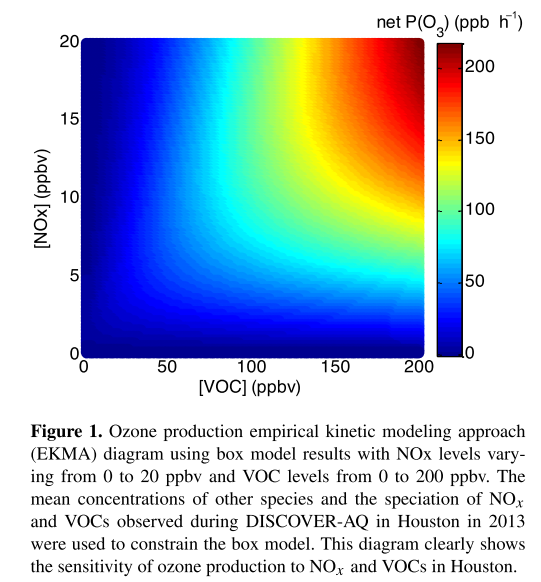
\includegraphics[width=.75\textwidth]{Figures/Mazzuca2016_NOxVOCOzone.png}
      \caption{Ozone production figure copied from \cite{Mazzuca2016}.}
      \label{LR:VOCs:fig_NOXVOCOzone}
    \end{figure}
      
    Isoprene is emitted and enters the atmosphere in the gas phase, where it reacts with various chemicals, forming many new chemicals with reactions at various time scales.
    One common compound which is produced by these reactions is HCHO, which is easier to measure and often used to estimate how much isoprene is being emitted.
    The estimated yield of HCHO is but one aspect of the many processes going on in this space.
    There are many reactions which occur and are important to capture in models due to their impacts on air quality and physical properties in the lower atmosphere.
    The many children processes and products which begin with isoprene oxidation are often called the isoprene (photochemical) cascade \cite{Crounse2012,Paulot2012,Wolfe2016}.
    
  \subsection{The isoprene cascade}
    \label{LR:VOCs:IsopCascade}
    
    Isoprene forms many products with various lifetimes, here I will present an overview of some important mechanisms which affect oxidation capacity, ozone and aerosol production.
    
    The primary first step for atmospheric isoprene is photooxidation, reacting with OH to form isoprene hydroxyperoxy radicals (ISOPOO, or ROO, or RO$\dot{O}$) (\cite{Wolfe2016,Marvin2017,Patchen2017}).
    More generally, photolysis and oxidation of many VOCs initially form alkyl radicals ($\dot{R}$).
    Alkene (VOCs with double bonded carbon) reactions with ozone lead to organic peroxy radicals (RO$\dot{O}$). 
    These go on to form many products and lead to (amongst other things) aerosol, formaldehyde, and ozone formation, depending on various other factors such as sunlight and NO pollution \citep{Atkinson2000}.
    There is still uncertainty about which pathways are most important following ISOPOO production: HO$_2$ reactions predominantly produce hydroxyhydroperoxides (ISOPOOH), NO reactions largely produce methyl vinyl ketone (MVK) and methacrolein (MCR), and RO$_2$ reactions are also possible \cite{Liu2016a}.
    
    
    The first step in oxidising alkenes (including isoprene) is a replacement by OH of a double bond, as summarised by the equation from \cite{Patchen2007}:
    % Uses package{mchem}
    \ce{R-CH=CH-R$^{\prime}$ + OH -> R-CH(OH)CH-R$^{\prime}$ }
    where R and R$^{\prime}$ represent hydrocarbons.
    This OH adduct then reacts with O$_2$ to produce a hydroxyperoxy radical (RO$\dot{O}$), which for isoprene can be any of six different isomers \citep{Patchen2007}.
    This is where the isoprene oxidation path splits depending on the NO$_X$ concentration.
    Reactions with NO can lead to ozone production in both isoprene and other non-methane organic compounds (NMOCs) and NMVOCs (\cite{Patchen2007,AtkinsonArey2003}).
    These reactions are complex and coupled, for example NO$_2$ concentrations can be increased by NMOC and NO reactions \citep{AtkinsonArey2003}.
    
    
    %% NO2 reaction -> PAN
    Reaction with NO$_2$ forms hydroxynitrate (RONO$_2$), also known as peroxyacetyl nitrate (PAN).
    The first generation of organic nitrates produced by isoprene oxidation range from 7\% to 12\%, shown in laboratory experiments \citep{Paulot2009a, Mao2013},
    A portion of isoprene nitrates are recycled back to NO$_X$, so may serve as a reservoir of nitrogen and allow its transport to the boundary layer of remote regions (\cite{Patchen2007,Paulot2009a}).
    \cite{Patchen2007} examine this branching step where isoprene either forms ROO or RONO$_2$, and for specific conditions they determine the reaction rates for each branch.
    They find the most frequent pathway is the formation of ROO (99.3\%).
    Although the PAN formation branch is quite minor, it can be very important.
    PAN can transport NO$_X$ to otherwise clean regions (\cite{Horowitz1998}), and can build up in the winter \citep{Lelieveld2009}.
    PAN has a relatively long lifetime (against OH, order of 1 day) and is able to transport and release the NO$_X$ in environments which are quite far from any emissions.
    This transport can be exacerbated by fast winds and low OH concentrations, which makes PAN an important factor in modelling atmospheric chemistry.
    
    
    The oxidation products of isoprene through OH adduction (forming ISOPOO) followed by addition of O$_2$ produces various isomers of alkylperoxyl radicals (organic peroxyl radicals, or RO$_2$), which react with HO$_2$ or NO and produce stable products (often called oxidised VOCs or OVOCs) \citep{Nguyen2014}.
    The ISOPOO radicals are eventually destroyed by NO, HO$_2$ and other RO$_2$, with most pathways potentially producing HCHO \citep{Wolfe2016}.
    Oxidation reactions are important and quickly stabilise the ratio of NO to NO$_2$. 
    NO$_X$ is removed primarily by conversion to nitric acid (HNO$_3$) followed by wet or dry deposition \citep{Ayers2006}.
    There is still large uncertainty around the fate of various RO$_2$ radicals, which limits understanding of the relative importance of some chemical processes \citep{Crounse2013}.
    
    Some portion of emitted isoprene leads to SOA, potentially through the formation of methacrylic acid epoxide (MAE) formed by decomposition of methacryloylperoxynitrate (MPAN, a second generation product of isoprene oxidation) as shown in smog chambers and field studies in \cite{Lin2013}.
    In the presence of NO$_X$, the ISOPOO radicals (RO$\dot{O}$) form organic nitrates after reacting with NO.
    Any organic nitrates which are formed affect levels of both HO$_X$ (H, OH, peroxy radicals) and NO$_X$, acting as a sink (\cite{Mao2013} and references therein).
    
    
    %% LOW NOX scenario
    Isoprene oxidation by OH is less well understood when lower concentrations of NO are present in the atmosphere.
    Initially isoprene was thought to be a sink for atmospheric oxidants \citep[e.g.][]{Guenther2000}.
    It was thought that in low NO environments, like those far from anthropogenic pollution and fires, oxidation of isoprene would create ISOPOOH and lead to low concentrations of OH and HO$_2$ \cite{Paulot2009b}.
    In \cite{Paulot2009b}, the HO$_X$ levels are shown to be largely unaffected by isoprene concentrations.
    They show that ISOPOOH is formed in yields $> 70\%$, and MACR and MVK is formed with yields $< 30\%$.
    The formation of MACR and MVK produces some HO$_X$, although not enough to close the gap.
    \cite{Paulot2009b} goes on to suggest (and provide experimental evidence) that dihydroxyperoxides (IEPOX) are formed from oxidation of the ISOPOOH, which form precursors for SOAs as well as closing the HO$_X$ concentration gap.
    They then use GEOS-Chem, modified to include IEPOX formation, to estimate that one third of isoprene peroxy radicals react with HO$_2$, and two thirds react with NO. 
    They estimated $95 \pm 45$\tgpyr IEPOX being created in the atmosphere, which (at the time) was not modelled by CTMs.
    Their work showed another pathway for isoprene based SOA creation, through these IEPOX creation and HO$_X$ recycling mechanisms.
    \cite{Peeters2010} suggested that the work of \cite{Paulot2009b} only partially bridges the gap between clean air HO concentration measurements and models.
    They suggested four new mechanisms for OH recycling in these pristine conditions.
    These can be summarised as OH regenerating reactions which occur during photolysis of hydroperoxy-methyl-butenals (HPALDs), and resulting photolabile peroxy-acid-aldehydes (PACALDs).
    These reactions are highly non-linear and subject to large uncertainty, however when compared against several campaigns they were shown to improve one particular models (IMAGES) HO$_X$ concentrations.
    In \cite{Crounse2012}, MACR products are examined in various conditions and hydroxy recycling is also observed in low NO conditions.
    
    Although understanding of OH production/recycling in these low NO conditions has been improved, many observations of OH are still quite under-predicted in models \citep{Mao2012}.
    \cite{Mao2012} showed how traditional OH measurements may be overestimated due to VOC oxidation.
    They looked at measurements in a remote forest in California and found that the instruments were generating OH internally.
    \cite{Nguyen2014} also see this VOC oxidation interference in measurements using a gas chromatographer (GC) with an equipped flame ionisation detector (FID).
    This lends more credence to the current understanding of VOC oxidation as it closed the gap between measurements and model predictions (\cite{Mao2012}).
       
    \cite{Peeters2010} showed that HO$_2$ is produced at near unity yields following isoprene oxidation initiated by HO.
    TODO: read more Peeters2010
      
    \cite{Nguyen2014} examine various measurement techniques to determine isoprene reactions in non-laboratory conditions.
    Thier work discussed how large uncertainties persist in isoprene oxidation, which carries through to predictions by atmospheric models.
    This work discussed how large uncertainties persist in isoprene oxidation, which carries through to predictions by atmospheric models.
    \cite{Nguyen2014} show preliminary estimates of low-NO yields of MVK and MCR to be 6$\pm3\%$ and 4$\pm2\%$ respectively, consistent with TODO:\cite{Liu2013}, but only when cold-trapping methods are employed.
    These yields each increase (due to interference by OVOCs) to greater than 40\% when directly sampled by GC-FID.
      
    % Night time stuff
    During the night isoprene is oxidised by NO$_3$ radicals, which joins to one of the double bonds and produces organic nitrates in high yield (65\% to 85\%) \citep{Mao2013}. (todo: read mao2013 para 3 cites)
    These organic nitrates go on to produce further SOAs, largely due to NO$_3$ reacting with first generation isoprene oxidation products \citep{Rollins2009}.
    \cite{Rollins2009} examine SOA production in a large chemical reaction chamber, over 16~hr in the dark and find first generation mass yield ($\Delta$SOA mass$/\Delta$isoprene mass) to be less than 0.7\%, with further oxidation of initial products (isoprene reacting twice with NO$_3$) yielding 14\%.
    This led to an overall mass yield of 2\% over the 16~hr experiment.
      
    Even with the recent boom in isoprene analysis, uncertainties remain in the isoprene oxidation mechanisms.
    Examples (taken from \cite{Nguyen2014}) include isoprene nitrate yields, which range from 4-15\% \citep{Paulot2009a}, 90\% disagreements in MAC and MVK yields TODO:\citep{Liu2013}, various possible sources for SOA TODO:\citep{Chan2010, Surratt2010, Lin2013}, unknown HPALD fates, incomplete O$_2$ incorporation TODO:\citep{Peeters2009,Crounse2013}, and under-characterized RO$_2$ lifetime impacts TODO:\citep{Wolfe2012}. TODO: get those citations and read abstracts.
    
    \subsubsection{Ozononlysis}
      Ozononlysis is the splitting of carbon chains by ozone molecules, and is among the primary oxidation pathway for volatile alkenes \citep{Nguyen2016}.
      Criegee intermediates (carbonyl oxides with two charge centres) are formed when isoprene reacts with O$_3$. 
      \cite{Nguyen2016} examine in detail a few of these, with proposed mechanisms for C$_1$ and C$_4$ Criegee intermediate reactions.
      The C$_1$ stabilised Criegee (CH$_2$OO, $\sim 61\%$) is therein proposed to react with water yielding $73\%$ hydroxymethyl hydroperoxide (HMHP), $6\%$ HCHO $+$ H$_2$O$_2$, and formic acid $+$ H$_2$O, and the same products with yields of 40, 6, and 54$\%$ respectively when this Criegee reacts with (H$_2$O)$_2$.
      TODO: more on Nguyen2016?
      
    \subsubsection{SOA}
      \label{LR:VOCs:IsopCascade:SOA}
      %% SOA production and overview?
      Gas phase emissions with higher vapour pressures can be oxidised into lower vapour pressure products which will partition between gas and particle phase, often called semi or non-volatile. 
 	    The aerosol products from these gas phase emissions (or the children thereof) are called SOA \citep{Kanakidou2005}.
      In the \cite{Kanakidou2005} review of global SOA science, uncertainty in radiative forcing of aerosols is highlighted, and 20-90~\% of PM mass in the lower troposphere is OA.
      Less volatile OA also plays a role, although PM production from this source is complicated and makes up only a small fraction ($\sim 1 \%$) of the resulting PM (\cite{Kroll2008, Bei2012}).
      Modelling OA has many uncertainties due to the complexity of SOA formation and various pathways such as aqueous phase oxidation which can significantly contribute to concentrations.
      This is further hindered by poor understanding of precursor emissions, and lumping together various compounds, of which only some form SOA (for example ORVOCs in GEIA (back in 2005)).
      Satellite data requires SOA models to estimate a full vertical profile of aerosols for remote sensing techniques \citep{Kanakidou2005}.
      
      SOA formation from VOCs in atmospheric CTMs is generally imperfect due to the complicated chemistry and diverse nature of atmospheric conditions.
      Yields of SOA from VOCs are often lumped together and based on empirical laboratory chamber data. 
      VOC oxidation was not feasible $\sim 12$ years ago (2005), as chamber studies did not extend over a large enough parameter range and the importance of heterogeneous aerosol chemistry on SOA formation was unquantified \citep{Kanakidou2005}.
      
      One of the large uncertainties with OA is the total effect on radiative forcing, 12 years ago it was well understood that most OA cool the atmosphere, with smaller particles having a larger affect due to the size matching the wavelengths of visible light \citep{Kanakidou2005}. 
      Transport and indirect effects complicate matters further, with cloud creation and modification of cloud properties being quite difficult to accurately predict.
      In the third IPCC report \citep{IPCC2001}, the uncertainty involved if OA forcing was a factor of 3 times the estimated effect. 
      This has since been improved however OA and cloud formation still remains a large uncertainty in more recent IPCC reports \citep{IPCC_Chapter2}.
      Figure \ref{LR:fig:IPCC_RF_AR4} shows the radiative forcing (RF) of various atmospheric constituents, it's clear that OA uncertainty dominates.
      Figure \ref{LR:fig:IPCC_RF_AR5} shows the same summary updated in chapter 8 of the fifth report, where the SOA uncertainty remains quite large.
      It's currently understood that SOA plays an indirect and complex role in cloud properties, with a net cooling effect \citep[Chapter 7,8]{IPCC_AR5_WG1}
      
      \begin{figure}
        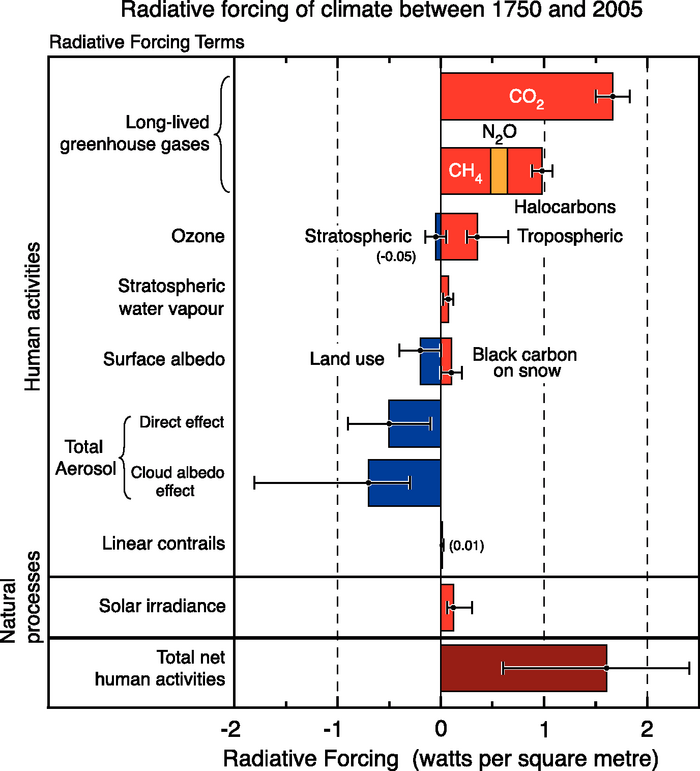
\includegraphics[width=\textwidth]{Figures/IPCC_WG1AR4_RFSummary.png}
        \caption{%
          The overall radiative forcings and uncertainties of several atmospheric constituents
  	      This is an image taken from \cite{IPCC_Chapter2}, found at \url{https://www.ipcc.ch/publications_and_data/ar4/wg1/en/faq-2-1.html}.}
        \label{LR:fig:IPCC_RF_AR4}
      \end{figure}
  
      \begin{figure}
        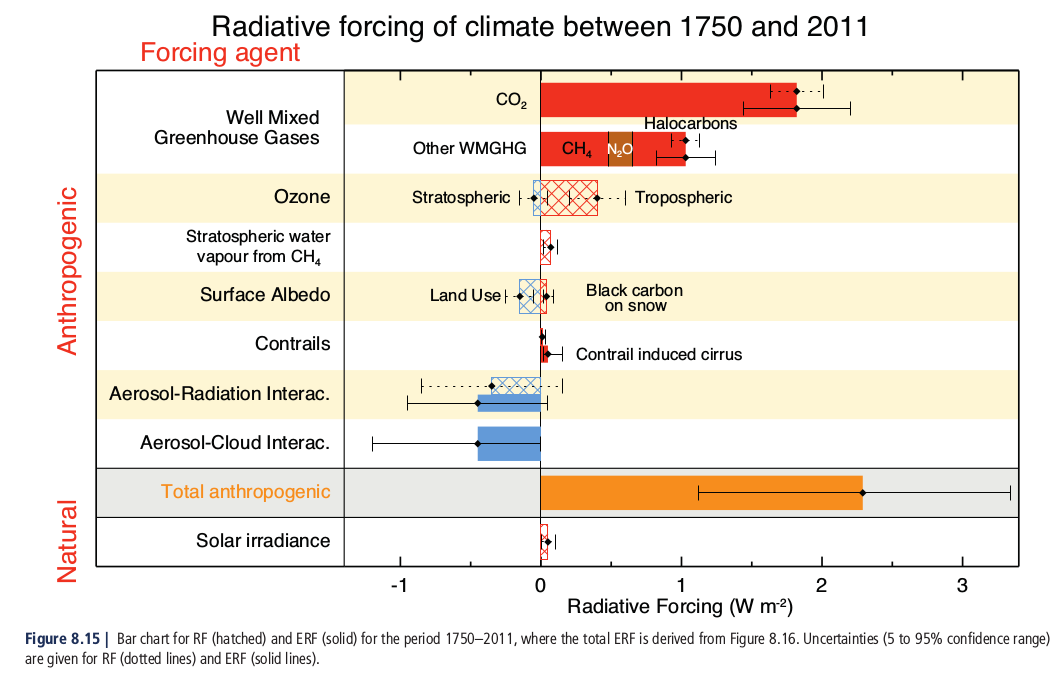
\includegraphics[width=\textwidth]{Figures/IPCC_WG1AR5_RFSummary.png}
        \caption{%
          The overall radiative forcings and uncertainties of several atmospheric constituents
  	      This is an image taken from \cite{IPCC_AR5_WG1}, chapter 8.}
        \label{LR:fig:IPCC_RF_AR5}
      \end{figure}    
      
      (TODO: read more of Kanakidou2005)
      The emissions of precursors to SOA was and is quite uncertain, in \cite{Kanakidou2005} they state that these uncertainties range from a factor of 2 to 5.
      They highlight emissions and flux measurements as well as implementing satellite data in models as a means of improving the emissions inventories.
      In 2005, (as of \cite{Kanakidou2005},) the knowledge gaps in isoprene and terpene oxidation processes included precursor gases to SOA, impact of NO$_X$ on SOA formation, heterogeneous reactions between particles and gaseous compounds, aqueous phase chemistry, and complete aerosol compositions.
      At this time SOA driven nucleation was under debate, as chamber studies showed that SOA led to new particles but only in the particle free laboratory setting. 
      Nucleation of new particles was suppressed by condensation if any seed aerosol was already present.
      Observed nucleation outside of laboratories was suggested to have arisen from biogenic SOAs, driven by ozonolysis.
      \cite{Kanakidou2005} concluded that it is very likely that organics contribute to particle growth and formation rates.
    
  \subsection{How and where do we measure them?}
    
    %% HOW its measured:
    
    \cite{Kanakidou2005} summarised the difficulty of chamber experiments used to measure isoprene reactions and the possible unsuitability of chamber study yields in the natural atmosphere.
    This is due to the complex relationship between NO$_X$, NO$_3$, OH, O$_3$, and the formation of aerosols being hard to attribute any single precursor.
    In \cite{Nguyen2014} many scientists and groups worked together on chamber measurements, to improve understanding of ambient atmospheric oxidation mechanisms of biogenic hydrocarbons (such as isoprene).
    %% CHAMBER study examples?
    
    
    % TODO: Campaigns
    TODO: Brief overview of all the measurement campaigns, pointing to Modelling and Data chapter for more details.
    There are relatively few measurements of isoprene in the southern hemisphere, including MUMBA(TODO CITE), other campaigns?, and very recently that girl from Macquarie University with an instrument in the daintree rainforest(TODO CITE, DESCRIBE?).
    For details on the MUMBA campaign see Section \ref{Model:Datasets:MUMBA}.
    An airflight campaign (HIPPO) measuring isoprene was also performed in 2009-2011? TODO: ask Jenny re this one.
    
    A particulate and air quality measurement campaign took place in Sydney using PTR-MS and GC-FID, for details see Section \ref{Model:Datasets:SPS}.
  
  
  \subsection{Emissions estimates}
    \label{LR:VOCs:EmissionsEstimates}
    
    %% HOW estimates are made
    There are two commonly used ways of estimating isoprene emissions, top-down or bottom-up.
    Bottom-up emission estimates generally model the flora and events which emit isoprene, like Eucalypts, factories, shrubs, etc.
    They use various properties of the emitters in order to estimate how much isoprene is being produced.
    Some of these properties include leaf areas, speciated responses to sunlight and temperature, moisture stress, etc (\cite{Guenther1995,Guenther2006}).
    Understanding how much isoprene is emitted, when and by what, is complicated.
    Since little data exists with which to verify many of these bottom-up emission inventories, they can be uncertain on a large scale.
    Emissions inventories such as MEGAN are bottom-up and use models of emissions based on tree types, weather, and other parameters.
    
    Top-down estimates look at how much of a chemical is in the atmosphere and try to work out how much of its major precursors were emitted.
    This generally takes advantage of longer lived products which may reach a measurable equilibrium in the atmosphere.
    For isoprene this is done by looking at atmospheric HCHO enhancement, which can be largely attributed to isoprene emissions once transport and other factors are accounted for.
    Recently \cite{Stavrakou2015} used satellite HCHO measurements to constrain anthropogenic sources of isoprene and found good global agreement with the bottom up estimates, although some regions had sources differ by up to 25-40\%. 
    Their study used the RETRO 2000 database for anthropogenic emission aprioris except for Asia in 2008 where REASv2 was used. 
    Since 1997, when GOME first measured HCHO over Asia \citep{Thomas1998}, satellites have been able to provide a total column measurement of HCHO, one of the primary products of isoprene.
    
    %% ESTIMATES
    It used to be thought that emissions of anthropogenic and biogenic VOCs (AVOCs, BVOCs respectively) were roughly similar (\cite{Muller1992}, TODO: more cites).
    Methane (CH$_4$) is one of the more abundant and potent VOCs, however it is often classified separately and compared against non-methane VOCs (NMVOCs).
    In the 1990's it became clear that biogenic emissions of VOCs were in fact dominant, although methane emissions are still largely anthropogenic. 
    The World Meteorological Organisation (WMO) estimated that we are emitting 360~Mt yr$^{-1}$ of methane, compared to biogenic emissions of around 200~Mt yr$^{-1}$ \citep{Atkinson2000}.
    In 1995 emissions of other VOCs were estimated at 1150~Mt yr$^{-1}$ (of carbon) from biogenic sources, and 100~Mt yr$^{-1}$ from anthropogenic sources \citep{Guenther1995, Atkinson2000}.
    These estimates were based on the MEGAN.
    It's remains clear that biogenic VOC (BVOC) emissions are far greater than anthropogenic emissions of VOCs, making up 87\% of NMVOC emissions \citep{Kanakidou2005, Kefauver2014}.
    Non methane BVOC emissions are estimated to be $\sim1150$\tgcpyr, of which isoprene (44\%) and monoterpenes (11\%) are the main single contributors (\cite{Guenther2000, Kefauver2014}). 
    
    \cite{Guenther2006} estimated that the Australian outback is among the worlds strongest isoprene emitters with forests in SE Australia having emission factors greater than 16 mg m$^{-2}$ h$^{-1}$ (see figure \ref{LR:O3andAQ:EmissionsEstimates:fig_MEGAN_EF}).
    Measurement campaigns in SE Australia have since cast doubt on the emission factors used by MEGAN, as the Eucalyptus trees and soil moisture were poorly studied \cite{Emmerson2016}.
    These emissions factor estimates are not well verified and measurements of isoprene (or other BVOC) emissions barely cover Australia either spatially or temporally.
    However, comprehensive coverage of one high yield product (HCHO) in the atmosphere over Australia exists in the form of satellite measurements.
    
    \begin{figure}
      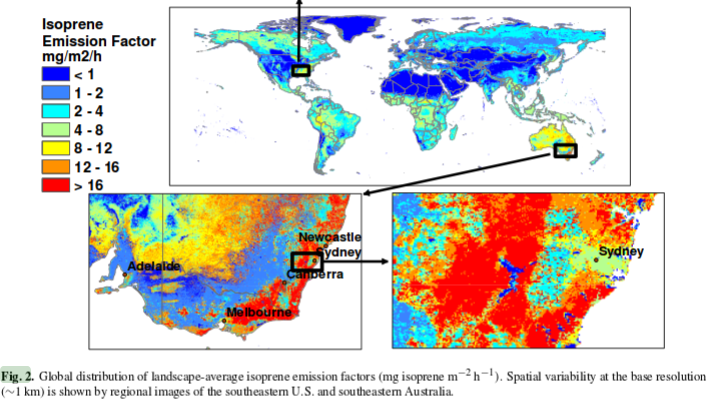
\includegraphics[width=\textwidth]{Figures/MeganIsoprene1.png}
      \caption{ Part of a figure from \cite{Guenther2006} showing global isoprene emission factors. }
      \label{LR:O3andAQ:EmissionsEstimates:fig_MEGAN_EF}
    \end{figure}
    
    % Uncertainties in estimates
    TODO:MOVE? (Uncertainties in estimates paragraph)
    Isoprene emissions estimates are still fairly uncertain, as global measurements are difficult and regional emissions can be very different. 
    %In 2005, Dr. C. Wiedinmyer et al. reviewed emissions inventories and showed %TODO 
    The global uncertainty of isoprene emission was estimated to be a factor of 2 to 5 (250-750\tgpyr) \citep{Kanakidou2005}.
    Improvements over the years have been incremental, and generally localised to regions of particular interest for air quality such as China and the USA TODO: find recent uncertainty estimate improvements examples.
    The lack of accuracy in BVOC emissions estimates prevents accurate determinations of the sources and distribution of pollutants including ozone and organic aerosols.
    Most of the tropospheric SOA comes from biogenic precursors, the evidence for this has grown over the last two decades \citep{Guenther1995, Kanakidou2005,Guenther2012}.
    Accuracy in VOC measurements is important: it has been shown that even the diurnal pattern of isoprene emissions has an effect on modelling ground level ozone \citep{Hewitt2011, Fan2004}.
    These uncertainties could explain why models of HCHO over Australia are poor at reproducing satellite measurements \citep{Stavrakou2009}.
    Over Australia specifically MEGAN has problems involving unpublished plant functional types and their emissions, as well as poorly optimised soil moisture parameterisation \citep{Emmerson2016}.
    Australia also lacks a clear estimate of emitted monoterpenes.
    \cite{Emmerson2016} suggest that monoterpenes may be emitted in similar quantites to isoprene, with more measurements required to determine if this is so.
    Their work suggests that MEGAN estimates of isoprene emissions may be 2-6 times too high, and monoterpene emissions $\sim3$ times too low over southeast Australia.
    
    
    It is important to note that many estimates of isoprene emission are based on a few algorithms which can depend greatly on input parameters (\cite{Arneth2008,Niinemets2010}).
    \cite{Arneth2008} argue that this monopoly of emissions estimates may be leading us to an incorrect understanding of isoprene chemistry.
    \cite{Yue2015} has shown that this is still a problem by looking at land carbon fluxes and modelling the sensitivity to VOC emissions estimates using two independent models of VOC emission.
    One model is photosynthesis based and estimates isoprene emissions using electron transfer energies and leaf physiology \citep{Niinemets1999}, while the other (MEGAN) uses the light and canopy temperature (\citep{Guenther1995,Arneth2007} TODO: Read Arneth et al., 2007; Unger et al., 2013).
    Both are sensitive to light and temperature parameterisations.
    
    Isoprene is hard to measure directly due to its short lifetime and weak spectral absorption, instead formaldehyde is often used as a proxy (\cite{Millet2006, Fu2007, Dufour2009, Marais2012, bauwens2013satellite, Kefauver2014, Bauwens2016}).
    This leads to another method of isoprene emissions estimation, termed top-down (as opposed to bottom-up estimates like MEGAN).
    
  
\section{Formaldehyde (HCHO)}
  \label{LR:HCHO}
  
  HCHO, aka methanal, methyl aldehyde, or methylene oxide, is of the aldehyde family.
  HCHO is an OVOC which is toxic, allergenic, and a potential carcinogen. 
  It is dangerous at low levels, with WHO guidelines for prolonged exposure at 80~ppb.
  HCHO is used as an adhesive in plywood, carpeting, and in the creation of paints and wallpapers.
  Emissions in enclosed spaces can build up to dangerous levels, especially if new furnishings are installed (\cite{Davenport2015}).
  At global scales HCHO in furniture is less important, as concentrations are driven by photochemical reactions with methane and other VOCs.
  
  In the remote troposphere HCHO production is dominated by methane oxidation, while in the continental boundary layer (CBL) production is largely due to NMVOCs (\cite{Abbot2003, Kefauver2014}).
  This suggests that HCHO enhancement over continents can be used to determine NMVOC emissions.
  In the CBL, HCHO enhancement is generally driven by short lived ($<1$~hr) precursors (such as isoprene and other VOCs).
  HCHO itself has a lifetime of a few hours (\cite{Kefauver2014}).
  
  \subsection{How HCHO is measured}
    % how to measure HCHO
    There are a few ways to measure HCHO, including Fourier Transform Infra-Red Spectrometry (FTIR) and Differential Optical Absorption Spectroscopy (DOAS).
    The DOAS technique takes advantage of the optically thin nature of HCHO in order to linearise the radiance differential through air masses with and without HCHO, using the Beer-Lambert intensity law.
    This method works for both in the home HCHO detection and global measurements from in-situ and remote sensing instruments (\cite{Guenther1995, Abad2015, Davenport2015}).
    As a trace gas HCHO interferes with light over a few wavelength bands, which allows instruments to detect concentrations between a known light source and a detector.
    Figure \ref{LR:fig:HCHOSpectrum} shows the interference spectrum of HCHO as well as a typical band used to examine interference in the DOAS technique.
    One difficulty is that this interference is relatively small (HCHO is optically thin) and other compounds absorb light at similar wavelengths (\cite{Davenport2015}).
    FTIR measurements can have a range of uncertainties, including systematic and random measurement errors and uncertain apriori shape factors and water profiles (eg: \cite{Franco2015}).
    Multiple axis DOAS (MAX-DOAS) uses DOAS over several open path directions and also examines the infra-red light interference.
    In \cite{Franco2015}, an FTIR spectrometer at Jungfraujoch is compared against both MAX-DOAS and satellite data, with two CTMs; GEOS-Chem and IMAGES v2 used to compare total columns and vertical resolution of each instrument.
    Generally satellites use a DOAS based technique, with chemical transport and radiative transfer models used to transform the non-vertical light path interference into vertical column amounts.
    
    \begin{figure}
      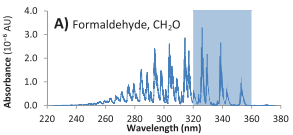
\includegraphics{Figures/HCHO/HCHOAbsorbanceDavenport.png}
      \caption{ %
        HCHO spectrum, with a typical band of wavelengths used for DOAS path measurements.
        This is a portion of an image from \cite{Davenport2015}.}
      \label{LR:fig:HCHOSpectrum}
    \end{figure}
    
    MAX-DOAS is a remote sensing technique which uses several DOAS measurements over different viewing paths.
    In these retrievals, the measurements of light absorption are performed over several elevations in order to add some vertical resolution to the measurement of trace gas concentrations.
    An example of this is shown in figure \ref{LR:HCHO:fig_MAXDOASExample}, which was taken from \cite{Lee2015}.
    Recently MAX-DOAS has been used to examine HCHO profiles in the clean free troposphere (\cite{Franco2015, Schreier2016}) as well as in polluted city air (\cite{Lee2015}).
    Depending on orography and atmospheric composition (ie. the influence of interfering chemicals), MAX-DOAS can be used to split the tropospheric column into two partial columns; giving a small amount of vertical resolution to HCHO measurements \citep[eg.]{Franco2015, Lee2015}.
    
    \begin{figure}
      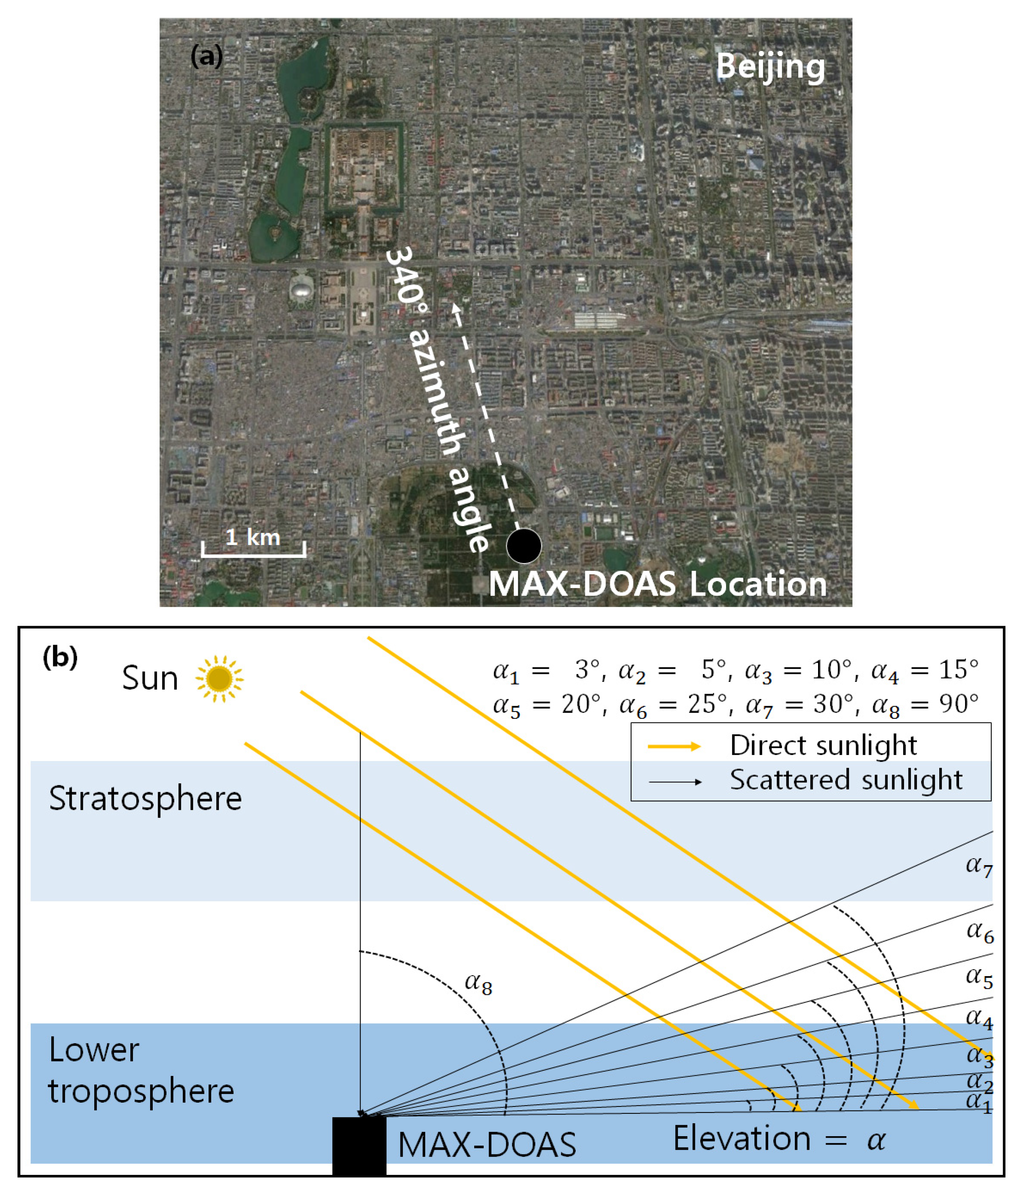
\includegraphics[width=\textwidth]{Figures/MAXDoasExample.png}
      \caption{ Image from \cite{Lee2015}.}
      \label{LR:HCHO:fig_MAXDOASExample}
    \end{figure}
    
    DOAS methods are based on light interference and absorption through air masses.
    Other types of measurement involve directly measuring the air, and determining chemical compounds through their physical properties.
    A proton transfer reaction mass spectrometer (PTR-MS) can be used to determine gas phase evolution of terpene oxidation products (\cite[eg.]{Lee2006a,Nguyen2014,Wolfe2016}).
    This is done through analysis of mass to charge ratios ($m/z$) of ionised air masses which are then identified as chemical compounds.
    \cite{Nguyen2014} use and compare several instruments (including one which is PTR-MS based) in the analysis of isoprene and monoterpene products.
    A Gas Chromatography mass spectrometer (GC-MS) is also able to identify isoprene, monoterpenes, and their products \cite[eg.]{Nguyen2014}.
    % TODO: Explain and find a couple of chamber studies to cite (should already be in my thing)
    
    Other measurement techniques include chromatographic and fluorimetric methods, both of which differ widely from each other and the spectroscopic methods (\cite{Hak2005}).
    \cite{Hak2005} examine a single air mass with 8 instruments using the four techniques (MAX-DOAS, FTIR, chromatographic, and flourimetric), and show that reasonable agreements can be achieved.
    Generally the measurements were somewhat close, the five Hantzsch instruments agreeing to within 11\% (after removing two potentially faulty measurements), although different calibration standards were used.
    Titration for the different calibration solutions could not be resolved, which may account for absolute offsets up to 30\%.
    These differences and non-uniformities between measurements (even among identical instruments) are part of the reason HCHO does not have a consistent network for global measurements like those for GHGs or Ozone (\cite{FortemsCheiney2012}).
  
  \subsection{Sources and sinks}
    \label{LR:HCHO:Sources}
    In the atmosphere HCHO is primarily produced through the oxidation of methane (CH$_4$) by the hydroxyl radical (OH).
    CH$_4$ concentrations are thought to be well constrained in models, with the ACCMIP comparison showing only $\sim3$\% inter-quartile range (\cite{Young2013}).
    Within the continental boundary layer, the major source of HCHO enhancement is VOC emissions reacting with OH radicals in the presence of NO$_X$ (\cite{Wagner2002, Millet2006, Kefauver2014}).
    There is a complex relationship between VOCs, HO$_X$, and NO$_X$, and with higher levels of NO$_X$ the speed that VOCs are converted into HCHO increases, as does the HCHO concentration (\cite{Wolfe2016}).
    Isoprene is the main VOC precursor of HCHO in the continental boundary layer, except near fires or anthropogenic sources of HCHO and precursors (\cite{Guenther1995, Kefauver2014, Wolfe2016}).
    
    Biomass burning (BB) can be a source of HCHO, and various other pollutants, precursors, and aerosols (\cite{Guenther1995, Andreae2001}).
    Additionally HCHO is emitted into the atmosphere directly through fossil fuel combustion, natural gas flaring, ethanol refining, and agricultural activity (\cite{Wolfe2016}).
    Background levels of HCHO are maintained by methane oxidation, while enhancements to regional and continental HCHO are largely driven by isoprene emissions (\cite{Guenther1995, Palmer2003, Shim2005, Kefauver2014}).
    \cite{Atkinson2000} summarised the background formation of HCHO with the following reaction:
    \begin{equation*} \label{LR:HCHO:Sources:eqn_MethaneBackground}
    OH + CH_4 (+ h\nu) + 2NO + 2O_2 \rightarrow OH + HCHO + H_2O + 2O_3
    \end{equation*}
    which shows that photolysis and oxidation of methane forms HCHO and ozone in a process that regenerates the OH radicals.
    
    Other terpenoids (monoterpenes, sesquiterpenes, etc.) can also produce HCHO, although generally to a lesser extent than isoprene, methane and biomass burning (\cite{Guenther2012}).
    Many of the HCHO yields from terpenoids are estimated through chamber studies which examine the products molecular mass and charge after mixing the compound of choice into a known volume of air (\cite[eg.]{Nguyen2014}).
    These conditions generally don't match those of the real world, where ambient air will have a cocktail of these compounds as well as various reactants.
    \cite{Nguyen2014} state that one of their goals is to recreate ambient atmosphere in their chamber studies with more accuracy, in order to improve interpretations and allow more accurate model parameters.
    An important factor in determining the yield of HCHO and other products from BVOCs is the local concentration of NO$_X$.
    \cite{Travis2016} show how modelled surface ozone is overestimated due to high estimates of  NO$_X$ emissions, which affect oxidative capacity and VOC reactions.
    
    %% HCHO SINKS
    HCHO has two major sinks, one being reactions with OH (oxidation), the other being photolysis: the process of being broken apart by photons (\cite{Crutzen1999, Wagner2002, Levy1972, Kefauver2014}).
    These reactions lead to a daytime lifetime of a few hours (\cite{Atkinson2000, Millet2006}).
    Both these loss processes (photolysis, oxidation) form CO and hydroperoxyl radicals (HO$_2$), and have global significance to radiative forcing and oxidative capacity (\cite{Franco2015}).
    The other notable sinks are wet and dry deposition, although these are not as significant (\cite{Atkinson2000}) (TODO: add more cites here).
    
    % Lead into satellite inversion
    In the past, HCHO levels were underestimated by models, often with large discrepancies, due to the poor understanding of methyl peroxy radical (CH$_3$OO) chemistry (\cite{Wagner2002}).
    Nowadays HCHO concentrations are better understood, however precursor emissions are one of the main unknowns (\cite[eg.]{Emmerson2016,Marvin2017}).
    \cite{Marvin2017} found that discrepancies in modelled HCHO concentrations are primarily due to second and later generation isoprene oxidation chemistry.
    
    Formaldehyde formed in the troposphere is mostly due to VOC (roughly one third each: methane, isoprene, others) oxidation.
    We can model this oxidation process in order to work out how much VOC is present based on the total HCHO.
    This requires among other things an idea of which VOCs are present and their yields of HCHO.
    The technique of determining isoprene emissions from satellite detected HCHO is called satellite inversion.
  
  \subsection{Satellite inversion}
    \label{LR:HCHO:SatelliteInversion}
    
    Satellites recording reflected solar spectra use Differential Optical Absorption Spectroscopy (DOAS) to measure various trace gases in the atmosphere, including formaldehyde. 
    Formaldehyde levels in the continental boundary layer are generally dominated by chemical formation due to VOC (largely isoprene) emissions \citep{Kefauver2014}.
    While satellite measurements can only be used during daytime hours, HCHO lifetimes are sufficiently short that any night-time chemistry will not affect midday observations \citep{Wolfe2016}.
    Satellites can be used to measure the seasonal and interannual variability of HCHO over Australia.
    These records can be compared with modeled estimates of HCHO and used as a proxy to estimate isoprene emissions.
    This has been done in North America \citep{Palmer2003, Millet2006}, South America, Africa, China, Europe \citep{Dufour2009}, and recently globally \citep{FortemsCheiney2012, Bauwens2016}.
    Often these works use two forms of measurement such as satellite and aircraft data combined for validation (\cite{Marais2014}).
    There is less information available from satellite measurements at higher latitudes due to increased errors (\cite{DeSmedt2015}).
    
    Using HCHO to determine emissions of isoprene was initially performed by \cite{Palmer2001, Palmer2003}, who used in-situ summertime HCHO measurements over North America as model validation.
    Isoprene emissions fluxes were derived using the Global Ozone Monitoring Experiment (GOME) satellite instrument.
    Palmer's method improved biogenic isoprene emissions estimates (compared with in-situ measurements) over two available inventories: the U.S. EPA Biogenic Emissions Inventory System (BEIS2) and the Global Emissions Inventory Activity (GEIA).
    This showed an inversion technique which could be used to improve large scale emissions estimates without further expensive measurement campaigns.
    
    Initially studies assumed a simple linear steady-state relationship between HCHO and it's precursors (\cite{Palmer2003, Palmer2006, Millet2006}).
    This allowed a simple calculation of isoprene using the measured HCHO, with estimated reaction rates and yields.
    The methodology for calculating VOCs from HCHO is laid out in \cite{Palmer2003}, and takes into account the expected lifetime and reaction rates of the precursor VOCs and HCHO.
    Assuming HCHO is produced quickly from short-lived intermediates, and the column is at steady state:
    \begin{eqnarray*}
      VOC_i \overset{k_i}{\rightarrow} Y_i HCHO
    \end{eqnarray*}
    Where $Y_i$ is HCHO yield per C atom (a measure of how much HCHO will form per gram of C from a VOC within a system), and $k_i$ is the reaction rate.
    Then assuming a steady state of atmospheric HCHO ($\Omega$ molecules $cm^{-2}$) produced by oxidation of VOCs (VOC$_i$) and no horizontal transport:
    \begin{eqnarray*}
      \Omega = \frac{1}{k_{HCHO}} \sum_{i} Y_i E_i
    \end{eqnarray*}
    Where i indexes a chemical species, $k_{HCHO}$ is the HCHO loss rate due to OH and photolysis, Y$_i$ is the molar HCHO yield from oxidation of i, and $E_i$ is emission fluxes ( C atoms $cm^{-2}s^{-1}$).
    
    Estimates of Y$_i$ can be attained from a model as shown in \cite{Millet2006}.
    This involves a reduced major axis (RMA) correlation calculation between modelled HCHO and isoprene columns, multiplied by their loss rates (to photolysis and oxidation) (as a normalising factor).  
    In high NOx environments where HCHO has a lifetime on the order of 30 minutes, it can be used to map isoprene emissions with spatial resolution from 10-100 kms.
    Horizontal transport 'smears' the HCHO signal so that source location would need to be calculated using windspeeds and loss rates (\cite{Palmer2001,Palmer2003}).
    Smearing is explicitly handled in these studies due to the importance of transport and NO$_X$ on forming robust and accurate estimates.
    Over Australia NO$_X$ levels are generally not high enough to ensure quick HCHO formation and we must take extra care that we can account for the transport or 'smearing' caused by slower HCHO formation, details on this process can be found in Section \ref{BioIsop:Methods:Smearing}.
    
    Another method of correcting isoprene emissions using observed HCHO total column involves a Bayesian inversion.
    \cite{Shim2005} work with GOME HCHO observations and GEOS-Chem, looking at areas with high signal to noise ratio (higher HCHO concentrations).
    They show that the model underestimates isoprene emissions and HCHO concentrations by 14-46\%, with the corrected VOC emissions reducing the model biases to 3-25\%.
    
    The Bayesian inversion is also used in \cite{Curci2010}, where a regional CTM (CHIMERE) simulates HCHO, which is compared against OMI observed HCHO and shown to be regionally biased.
    This bias is expected to be caused by errors in MEGANs isoprene emissions estimations.
    The CHIMERE model is used to derive yields of HCHO from the various local VOCs and these are then used in estimating local emissions.
    The model is run initially with emissions of BVOCs and reactive anthropogenic VOCs (RAVOCs) turned off in order to work out the background (b) values of these compounds.
    The Bayesian inversion is used to correct regionally biased biogenic isoprene emissions by optimising these parameters in order to simulate HCHO closest to the observed HCHO levels.
    \cite{Curci2010} uses CHIMERE as the forward model to determine the relationship between HCHO (y), isorene and reactive anthropogenic VOCs (\textbf{x}), using 
    \begin{equation}
    y=\mathbf{K}x + b + \epsilon
    \end{equation}
    where $\epsilon$ are the (assumed) independent errors in measurements.
    K is the Jacobian matrix determined from CHIMERE representing the sensitivity of y to the state variable x.
    This K matrix is used in conjunction with error covariance in x to determine the Maximum A Posteriori (MAP) solution to calculate the optimal estimate of x ($\hat{x}$).
    
    %TODO
    TODO: Read through this list of sources on the hcho to isop process : taken from Wolfe2015
    Such techniques have informed isoprene emission inventories in North America (Abbot et al., 2003; Millet et al., 2008 (\cite{Palmer2003,Millet2006,Palmer2006})), South America ((\cite{Barkley2013}), 2008), Europe (\cite{Curci2010,Dufour2009}), Africa (\cite{Marais2012}), Asia (Fu et al., 2007; Stavrakou et al., 2014), and globally (Fortems-Cheiney et al., 2012; (\cite{Shim2005}); Stavrakou et al., 2009).
    
    
    More recently, full inversions that better account for transport, source attribution, and chemical schemes have been implemented (\cite{FortemsCheiney2012}).
    TODO: full description of this better inversion technique going through FortemsCheiney2012.
    
    Validation is important due to the various uncertainties in the satellite remote sensing process, with apriori assumptions having the greatest effect on structural uncertainty between measurements techniques \cite{Lorente2017}.
    \cite{Zhu2016} use SEAC$^4$RS aircraft HCHO measurements over the southeastern US as model validation, and show a bias in the assumed OMI shape factor that leads to a bias between satellite and SEAC$^4$RS measurements.
    \cite{Marais2014} compare OMI based isoprene emission estimates against relaxed eddy accumulation measurements from African field campaigns, as well as MEGAN and GEOS-5 inventories.
    \cite{Dufour2009} use HCHO from SCIAMACHY, and examine Europe using CHIMERE as the chemical model. 
    In their work they show that satellite measurements can reduce source emission uncertainty by a factor of two, where emissions are relatively large.
    
    
    \cite{Kefauver2014} reviews remote sensing of BVOCs, which are on the rise, examining the last 20 years of data and analysis of the satellite products.
    Their review encompasses the latest reports up to 2014
    The modelled isoprene and BVOC emissions from MEGAN \citep{Guenther2000} of 500 and 1150~Tga$^{-1}$ respectively are still the global go to estimates.
    Their review reinforces the message that NMVOCs affect the oxidative capacity of the atmosphere and are largely driven by and sensitive to vegetation.
    The tropospheric affects from NMVOCs on the hydroxyl radical (OH), ozone (O$_3$), SOAs, and methane longevity, all interconnect to form a very complex system which still suffers from relatively large uncertainties in both measurement and chemistry mechanisms.
    One focus of \cite{Kefauver2014} is HCHO, which is the dominant product of most BVOCs which is measurable by remote sensing.
    The main datasets of HCHO are from four satellite instruments: GOME on ERS-2, SCIAMACHY on ENVI-SAT, OMI on EOS AURA, and GOME2 on MetOp-A.
    These satellites have slightly different spectral and spatial resolutions, as well as using varied processes to estimate HCHO from detected radiances.
    This can lead to different estimates between instruments or methodologies as described in \cite{Lorent2017}, which means validation and comparison is more important when using these remotely sensed data.
    
    Total HCHO is measured by satellite over the entire world, however the technique is not perfect and suffers from uncertainties and interferences.
    Satellite based chemical concentrations rely on ground-based measurements and modelled data for validation.
    They provide various readings with daily global coverage which is not otherwise feasable.
  
  \subsection{Satellite HCHO detection}
    \label{LR:HCHO:SatelliteDetection}
    TODO: Refactor this section so it's readable
    
    Several satellites provide long term trace gas observations with near complete global coverage, including the ERS-2 launched in April 1995 which houses the GOME ultraviolet and visible (UV-Vis) spectrometer, the AURA launched in July 2004 which houses the OMI UV-Vis spectrometer, the MetOp-A and B launched in October 2006 and September 2012 respectively both housing a GOME-2 UV-Vis spectrometer.
    These satellites are on Low Earth Orbit (LEO) trajectories and overpass any area up to once per day.
    Satellites can use DOAS techniques with radiative transfer calculations on solar radiation absorption spectra to measure column HCHO .
    An example of a spectrum retrieved from the GOME-2 instrument is given in figure \ref{LR:HCHO:SatelliteDetection:fig_GOME_products}.
    Measurements done using DOAS often apply a forward radiative transfer model (RTM) such as LIDORT in order to determine a trace gas's radiative properties at various altitudes.
    
    \begin{figure}
      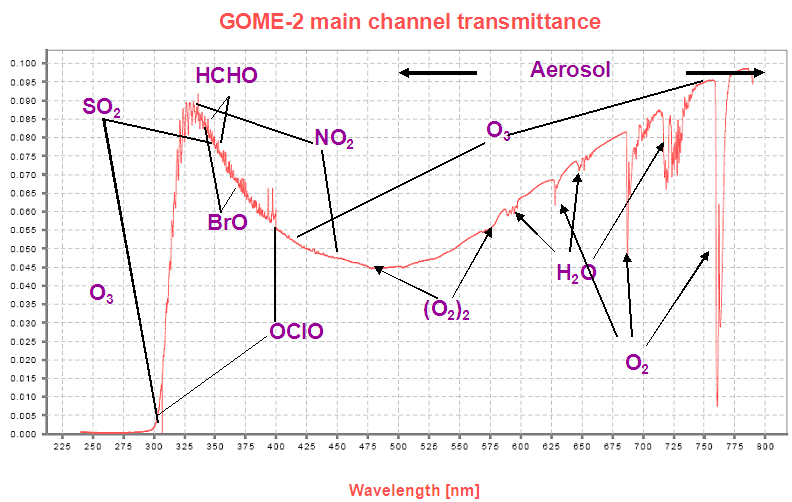
\includegraphics[width=\textwidth]{Figures/GOME_SPECTRUM.jpg}
      \caption{An example spectrum showing interferences used for species concentration measurements by GOME-2. Image by EUMETSAT and ESA (\cite{GOME2Image}.})
      \label{LR:HCHO:SatelliteDetection:fig_GOME_products}
    \end{figure}
    
    Satellites record near nadir (vertical) reflected spectra between around 250-700~nm split into spectral components at around $0.3$~nm in order to calculate trace gases including O$_3$, NO$_2$, and HCHO (eg: \cite{Leue2001}).
    Several public data servers are available which include products from satellites, including NASAs Earthdata portal (\url{https://earthdata.nasa.gov/}) and the Belgian Institute for Space Aeronomy (IASB-BIRA) Aeronomie site (\url{http://h2co.aeronomie.be/}).
    
    
    Instruments including MODIS on board the AQUA and TERRA satellites are able to determine aerosol optical depth (AOD), a measure of atmospheric scatter and absorbance. 
    An AOD of under 0.05 indicates a clear sky, while values of 1 or greater indicate increasingly hazy conditions.
    This is an important atmospheric property allowing us to track dust storms and pollution events as well as determine where measurements from other instruments may be compromised by high interference.
    Satellite measured AOD requires validation by more accurate ground based instruments like those of AERONET which uses more than 200 sun photometers scattered globally. 
    
    \subsubsection{OMI measurements}
    
      The OMI instrument on board AURA has been active since July 2005, it records spectra from 264-504~nm using an array of 60 detectors with mid-resolution (0.4-0.6~nm).
      This band of wavelengths allows measurments of trace gases including O$_3$, NO$_2$, SO$_2$, HCHO, and various other quantities like surface UV radiation.
      Recently \cite{Schenkeveld2017} analysed the performance over time of the instrument and found irradiance degradation of 3-8\%, changed radiances of 1-2\%, and a stable wavelength calibration within 0.005-0.020~nm.
      They also provide a very nice summary of the OMI instrument copied here in Fig. \ref{LR:HCHO:SatelliteDetection:fig_Shenkeveld_OMI_summary}, as it shows the instruments spectral, temporal, and spatial resolutions.
      These changes are measured excluding the row anomaly (RA) effect, which is relatively stable since 2011, although it is still growing and remains the most serious concern.
      An analysis of the row anomaly by \cite{Huang2017} state that OMI ozone columns remain suitable for scientific use, with recommendation for further evaluation.
      And analysis of OMI output by \cite{Schenkeveld2017} concludes that data is still of high quality and will deliver useful information for 5-10 more years, with radiances only changing by $1-2\%$ outside of RA impacted areas.
      The RA began in June 2007, with some cross-track rows seemingly blocked. The most likely cause is some instrument insulation partially obscuring the radiance port (\cite{Schenkeveld2017}).
      
      \begin{figure}
        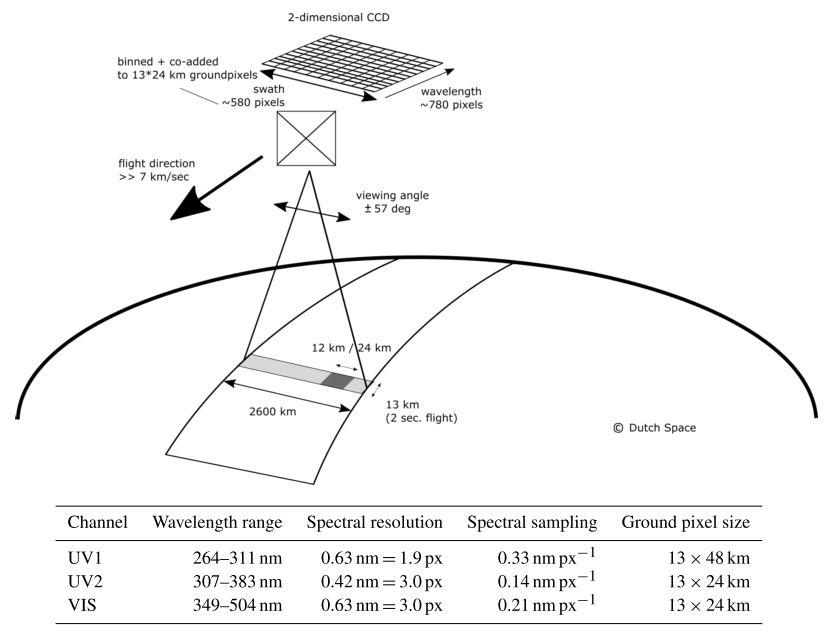
\includegraphics[width=\textwidth]{Figures/Shenkeveld_OMI_summary.png}
%        \caption{ %
%          Figure 1 and Table 1 from \cite{Schenkeveld2017}, with the following caption ``An impression of OMI flying over the Earth. The spectrum of a ground pixel is projected on the wavelength dimension of the charge-coupled device (CCD; the columns). The cross-track ground pixels are projected on the swath dimension of the CCD (the rows). The forward speed of 7~kms$^{-1}$ and an exposure time of 2~s lead to a ground pixel size of 13~km in the flight direction. The viewing angle of 114\degr leads to a swath width on the ground of 2600~km.''
%          The table shows the optical properties for OMIs three channels.}
        \label{LR:HCHO:SatelliteDetection:fig_Shenkeveld_OMI_summary}
      \end{figure}
      
      Soon even more HCHO data will be available in the form of geostationary satellite measurements (\cite{Kwon2017}).
      \cite{Kwon2017} examine simulated geostationary measurements against GEOS-Chem column simulations to determine the most important instrument sensitivities.
      Geostationary satellites can provide temporally rich measurements over an area, as they are not sweeping around the earth but fixed relative to one latitude and longitude.
    
    
    \subsubsection{DOAS}
      TODO: some of this is repeated in isoprene chapter satellite section.
      
      The DOAS technique uses solar radiation absorption spectra to measure trace gases through paths of light.
      The RTM used in DOAS techniques is based on Beer's law relating the attenuation of light to the properties of the medium it travels through.
      Beer's law states that $ T = I/I_0 = e^{-\tau} $ with T being transmittance, $\tau$ being optical depth, and I, I$_0$ being radiant flux received at instrument and emitted at source respectively.
      From $ \tau_i = \int \rho_i \beta_i ds $ we get:
      $$ I = I_0 \exp {\left( \Sigma_i \int \rho_i \beta_i ds \right) } $$
      Where i represents a chemical species index, $\rho$ is a species density(molecules per cm$^3$), $\beta$ is the scattering and absorption cross section area (cm$^2$), and the integral over ds represents integration over the path from light source to instrument.
      The forward RTM used for satellite data products also involves functions representing extinction from Mie and Rayleigh scattering, and the efficiency of these on intensities from the trace gas under inspection, as well as accounting for various atmospheric parameters which may or may not be estimated (e.g. albedo).
      
    \subsubsection{AMF}
      To convert the trace gas profile from a reflected solar radiance column (slanted along the light path) into a purely vertical column requires calculations of an air mass factor (AMF).
      In satellite data, the AMF is typically a scalar value for each horizontal grid point which will equal the ratio of the total vertical column density to the total slant column density.
      This value should also account for instrument sensitivities to various wavelengths at various altitudes, and is unique for each trace gas under consideration.
    
      An AMF characterises measurement sensitivity to a trace gas at various altitudes \cite[e.g.]{Palmer2001}.
      \cite{Lorente2017} show that AMF calculations can be the largest source of unertainty in satellite measurements.
      Another way of describing AMFs are as measures of how radiance at the top of the atmosphere (TOA) changes with trace gas optical depths at specific altitudes (\cite{Lorente2017}).
      Calculation of the AMF is important as it is multiplied against the estimated slant columns in order to give vertical column amounts.

      Related to the AMF is the averaging kernal (AK), which is used to handle instrument measurements which are sensitive to concentrations at different altitudes in the atmosphere.
      DOAS methods can be heavily influenced by the initial estimates of a trace gas profile (the apriori) which is often produced by modelling, so when comparing models of these trace gases to satellite measurements extra care needs to be taken to avoid introducing bias from differing apriori assumptions.
      One way to remove these apriori influences is through the satellites AK (or by using AMFs), which takes into account the vertical profile of the modelled trace gas and instrument sensitivity to the trace gas (\cite{Eskes2003, Palmer2001}).
      % TODO read and note this paper:
      \cite{Lamsal2014} recommends that when comparing satellite data to models, the AMF should first be recalculated using the model as an apriori.
      This is in order to remove any apriori bias between model and satellite columns.
    
    \subsubsection{Satellite uncertainties}
      %% grid size and averaging
      Satellite measurements of HCHO are relatively uncertain, however this can be improved by averaging over larger grid boxes or longer time scales.
      An example of this can be seen in \cite{Dufour2009}, where monthly averaging is used to decrease the measurements uncertainty.
      They examine HCHO in Europe, which is low; near the detection limit of satellite measurements.
      Taking monthly averages allows enough certainty that useful inversions can be determined to estimate the source emissions of HCHO.
      The finer nadir resolution of OMI (13 by 24~km${^2}$) compared to other satellites reduces cloud influence (\cite{Millet2006, Millet2008}). 
      Although the uncertainty in each pixel is $\sim 2 \times 10^{16}$, which is $5 \times$ higher than GOME, there are $\sim 100-200 \times $ as many measurements due to the smaller footprint and better temporal resolution of OMI, which allows a greater reduction of uncertainty with averaging (\cite{Chance2002,Millet2008}).
      
      %% SURFACE CONDITIONS AND CLOUDS
      In cloudy, hazy or polluted areas measurements are more difficult to analyse (\cite[e.g.][]{Palmer2003,Marais2014}).
      Recent work by \cite{Vasilkov2017} showed that updating how the surface reflectivity is incorporated into satellite measurements can change the retrievals by 50~\% in polluted areas.
      
      %% BACKGROUND MEASUREMENTS
      In satellite HCHO products, concentrations over the remote pacific ocean are sometimes used to analyse faulty instrument readings.
      This is due to the expected invariance of HCHO over this region.
      For instance GOME (an instrument which measures trace gases on board the ERS-2) corrects for an instrument artifact using modelled HCHO over the remote pacific (\cite{Shim2015}).
      OMI HCHO products use a similar technique to account for sensor plate drift and changing bromine sensitivity (\cite{Abad2015})
      
      
      %% EXAMPLES OF BIAS
      For many places the tropospheric column HCHO measured by satellite is biased low, \cite{Zhu2016} examine six available datasets and show a bias of 20 - 51\% over south east USA when compared against a campaign of aircraft observations (SEAC$^4$RS).
      \cite{DeSmedt2015} also found a low bias from 20 - 40\% when comparing OMI and GOME2 observations against ground based vertical profiles, and \cite{Barkley2013} determine OMI to be 37\% low compared with aircraft measurements over Guyana.
      These bias can be corrected by improving the assumed apriori HCHO profiles which are used to calculate the AMFs of the satellite columns.
      \cite{Millet2006} examine OMI HCHO columns over North America and determine overall uncertainty to be 40\%, with most of this coming from cloud interference.
      \cite{Millet2008} shows that there also exists some latitude based bias, as well as a systematic offset between the OMI and GOME instruments.
      This does not appear to be due to the different overpass times of the two instruments.
      
      %% UNCERTAINTY CALCULATIONS
      Uncertainty in the OMI satellite instrument is calculated by the Smithsonian Astrophysical Observatory (SAO) group using the uncertainty in backscattered radiation retrievals (\cite{Abad2015, Abad2016}).
      Another method of calculating the uncertainty is used by the Belgian Institute for Space Aeronomy (BIRA) group, who determine uncertainty from the standard deviation of HCHO over the remote pacific ocean \citep{DeSmedt2012, DeSmedt2015}.
      
      A full analysis of the AMF uncertainty in OMI measurements, as well as the structural uncertainty (between different systems of calculations applied to the same data) is performed by \cite{Lorente2017}.
      They determine the structural uncertainty using ensemble techniques on seven AMF calculation approaches used by different retrieval groups.
      They show that in scenarios where the gas is enhanced in the lower troposphere, AMF calculation is the largest uncertainty in satellite measurements.
      In polluted environments the structural uncertainty is estimated at 42~\%, or 31~\% over unpolluted environments.
      The importance of apriori and ancilliary data (such as surface albedo and cloud top height) is also shown, as it sharply affects the structural uncertainty.
      
      GOME suffers from similar uncertainties to OMI, as the same general method of DOAS remote measurements are performed.
      The uncertainty from slant column fitting has been calculated for GOME to be $4\times10^{15}$ molecules cm$^{-2}$ \citep{Chance2000, Millet2006}. 
      The conversion factor for slant to vertical columns (AMF) calculation also suffers from errors; primarily from surface albedo, HCHO vertical profile apriori, aerosol, and cloud influence \citep{Millet2006}. 
      AMF uncertainties for GOME are calculated to be $1$ to $1.3\times10^{15}$ molecules cm$^{-2}$ by \cite{Shim2005}.
    
    
  \subsection{Glyoxyl TODO: move somewhere fitting?}
  
    Another chemical retrievable from satellite observation is Glyoxyl, which can be used to further determine what sort of precursors to HCHO are being emitted \citep{Stavrakou2009, Miller2014, Miller2017}.
    TODO: go through 2014 paper and see if it's easy to retrieve, then email Dr. Chris Miller.
    For example \cite{Cao2018_discuss} recently used Glyoxyl measurements to improve understanding of biogenic and anthropogenic NMVOC emissions over China.
    This involved using a method pioneered by \cite{Stavrakou2009} TODO: get this cite and check method out.
   
    Glyoxyl (CHOCHO) is important to us as it shares many properties with HCHO, and may provide additional information in determining isoprene emissions.
    Glyoxyl is another product of VOC oxidation in the atmosphere, with isoprene being the main source globally.
    Under high NO$_X$ conditions, glyoxyl forms rapidly, similarly to HCHO.
    However, glyoxyl also forms in low NO$_X$ environments both slowly (through isoprene epoxydiols), and rapidly (through di-hydroperoxide dicarbonyl compound photolysation \citep{Crounse2013}.
    This process is similar to the proposed mechanisms for hydroperoxyaldehydes by \cite{Peeters2014} and carbonyl nitrates \citep{Muller2014}.
    Aromatics which are largely anthropogenic form glyoxyl quickly, while HCHO is produced slower, allowing determination of anthropogenic sources \citep{Cao2018_discuss}.
    
    HCHO has been used to estimate isoprene emissions (some examples in Section \ref{LR:HCHO:SatelliteInversion}) but many uncertainties exist.
    One of these uncertainties is the yield of HCHO from isoprene, especially in low NO$_X$ environments.
    Glyoxyl could prove complementary to HCHO in constraining isoprene emissions (TODO: Read and cite Vrekoussis2009,2010, Chan Miller 2014, Alvarado 2014) \citep{Miller2017}.
    Recently \cite{Miller2017} updated GEOS-Chem to include the prompt formation of glyoxyl and compared this with satellite and airplane measurements over the USA.
    Glyoxyl is formed by isoprene oxidation rapidly in low NO$_X$ conditions, unlike HCHO.
    With coming geostationary satellites, which provide greater time resolved measurements of HCHO and CHOCHO, this mechanism could be used to clearly show when low NO$_X$ isoprene chemistry is being undertaken \citep{Miller2017}.
    
\section{Models}
  \label{LR:Models}
  \subsection{How can models help}
    
    Models can fill the gaps (both spatial and temporal) in measurement records, and are used to predict/avoid/mitigate hazardous scenarios.
    They are used ideally to steer us away from unsustainable pollution and help complete our understanding of the world from small to large scales.
    They can be used to increase measurement accuracy (for instance in satellite measurements) and determine where we lack information, while also checking the performance of new instruments.
    Precisely representing various chemicals and reactions in the atmosphere allows efficient mitigation of pollution, since we can compare scenarios against one another.
    Currently, improved isoprene understanding is critical for effective air quality measuring \citep{Marvin2017}.
    
    Chemical Transport Models (CTMs) simulate production, loss, and transport of chemical species.
    This is generally calculated using one or both of the Eulerian (box) or Lagrangian (puff) frames of reference.
    CTMs normally solve the continuity equations simultaneously with chemical production and loss for chemicals under inspection. 
    The continuity equations describe transport of a conserved quantity such as mass, which, solved together with production and loss of a chemical can provide detailed simulations of natural processes.
    Models provide a simulation of chemical densities and transport over time as a model runs.
    The general continuity equation links a quantity of a substance (q) to the field in which it flows and can be described by the formula:
    \begin{eqnarray*}
      \frac{\partial \rho}{\partial t} + \nabla \cdot j &=& \sigma 
    \end{eqnarray*}
    where $\rho$ is density of q in the field, t is time, $\nabla$ is divergence, j is the flux (q per unit area per unit time entering or leaving the field), and $\sigma$ is the generation or loss of q per unit volume per unit time.
    
    
    The type of model best suited to modelling the entire earth uses the Eulerian frame of reference, where the atmosphere is broken up into 3-D boxes with densities and transport calculated and stored for sequential steps in time at each location.
    The mass balance equation must be satisfied in any realistic long term box model and is as follows: 
    \begin{align*}
      \frac{dm}{dt} &=& \sum{sources}-\sum{sinks} \\
      &=& F_{in} + E + P - F_{out} - L - D 
    \end{align*}
    where m is mass of a chemical, E and D are emission and deposition, P and L are production and loss, and F is chemical transport in and out, as shown in figure \ref{LR:Models:fig_boxmodel}.
    Many chemical species interact with each other through production and loss. 
    Any large chemical model will solve this mass balance equation over highly coupled arrays of partial differential equations which can be complex and time consuming.
    
    \begin{figure}
      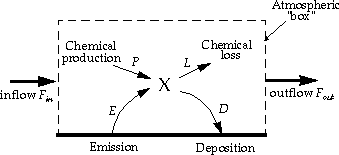
\includegraphics{Figures/boxmodel.png}
      \caption{ %
        Standard box model parameters, image taken from \cite{Jacob_1999_book}. }
      \label{LR:Models:fig_boxmodel}
    \end{figure}
    
    In many CTMs the isoprene emissions are calculated seperately using MEGAN, and then used as boundary conditions (EG: \cite{Guenther2006}). 
    This can speed up calculations as the transport and concentrations can be simulated in various conditions without recalculating the emissions.
    Trace gases with short lifetimes and complex chemistry such as isoprene are often hard to measure which makes verifying model estimates difficult.
    Contemporary models generally use mathematical differential solving tools of various complexity to solve chemical equations and reaction rates (often called chemical mechanisms) in order to predict an environments evolution over time.
    Different solvers may be slower or faster and more suited to particular situations based on the stability of the equations and systems involved, and chemical mechanisms may vary in how many reactions and chemicals are listed and grouped together.
    For example: Since [O] $<<$ [O$_3$] the chemical family O$_X$ (  O$_X \equiv $ O $+$ O$_3$ ) can be used to simplify chemistry simulations and approximate O$_3$ concentrations \citep[][Chapter 3]{BrasseurJacob2017}.
    \cite{Zhang2012} examine the outputs from a regional model (WRF/Chem) using three different chemical mechanisms, and they show that particulate matter prediction is sensitive to the choice of chemical mechanism. 
    
  \subsection{Relevant model frameworks}
  \label{LR:Models:frames}
    
    % Outline of ACM
    Atmospheric chemistry models (ACMs) require various inputs and can be sensitive to ozone and oxidative parameterisations. 
    TODO: read more Christian 2017,
    TODO: put some more generic ACM info here.
    
    \subsubsection{Box models} 
    \label{LR:Models:frames:box}
    % for example CAABA/MECCA
      A box model involves modelling chemistry in a singular set of conditions without transport or any spatial gradients.
      One box model used in this thesis is called CAABA/MECCA, and is described here as an example.
      
      CAABA (Chemistry As A Boxmodel Application) estimates the chemical concentrations accounting for J-values (JVAL), simplified and parameterised photolysis (SAPPHO) and simplified emission and depositions (SEMIDEP).
      CAABA runs in a single scenario (or box) with given emissions, depositions, and initial concentrations, allowing the examination of chemistry in a very specific environment to be modelled with high temporal resolution.
      This has been used with an atmospheric chemistry model MECCA (Module Efficiently Calculating the Chemistry of the Atmosphere) which implements tropospheric and stratospheric chemistry for both the gas and the aqueous phases \citep{Sander2005}.
      MECCA chemical mechanisms include basic O$_3$, CH$_4$, NO$_X$, and HO$_X$ chemistry, as well as non methane hydrocarbon (NMHC) chemistry, considering gas phase, aqueus phase, and heterogenous reactions. \citep{Sander2005}
      For the numerical integration, MECCA uses the KPP software (\cite{SanduSander2006}), which takes chemical reactions and their rate coefficients and codes integral solutions to the system.
      The combination of the CAABA box model with MECCA module is called CAABA/MECCA and is currently at version 3.
      CAABA/MECCA been implemented for various calculations including ozone chemistry throughout the atmosphere in \cite{Zanis2014}.
  
      MECCA could also be used as the chemistry mechanism for a more complex, 3-dimensional model (\cite[e.g.][]{Jockel2006}).
      The connection is established via the MESSy interface (\url{http://www.messy-interface.org}) developed by \cite{Jockel2005} as part of an effort to simplify the framework for modelling the atmospheres at various scales.
      The user manual is available online at \url{http://www.rolf-sander.net/messy/mecca/caaba_mecca_manual.pdf}.
  
      By allowing for interactions between boxes this concept can be extended to multiple-box models.
      These are simply multiple instances of single boxes with the addition of transport between them, which generally requires a meteorological model to provide winds, and other transport mechanisms.
      
    \subsubsection{Chemical transport} %% eg. GEOS-Chem
      GEOS-Chem is an example of this, with many boxes covering the globe, each with chemistry and dynamic meteorological conditions.
      The transport between boxes also needs to be taken into account when simulating concentrations.
      Additionally the different meteorological conditions such as wind and air pressure need to be handled within each box.      
      GEOS-Chem has a meteorological model coupled to a chemical model, which simulates the world in a three dimensional grid of connected boxes.
      
      GEOS-Chem is a well supported global, Eulerian CTM with a state of the science chemical mechanism, with transport driven by meteorological input from the Goddard Earth Observing System (GEOS) of the NASA Global Modeling and Assimilation Office (GMAO).
      GEOS-Chem simulates more than 100 chemical species from the earth's surface up to the edge of space (0.01~hPa) and can be used in combination with remote and in-situ sensing data to give a verifiable estimate of atmospheric gases and aerosols.
      It was developed, and is maintained, by Harvard University staff as well as users and researchers worldwide.
      Several driving meteorological fields exist with different resolutions, the finest at 0.25 by 0.3125$^\circ$ horizontally at 5 minute time steps with 72 vertical levels.
      
      Global CTMs are often run using one or several emission models (or the output from them) to determine boundary conditions for many gridboxes.
      TODO: is this the case? Doesn't GEOS-Chem have coupled chemistry and meteorology? Check the wiki.
      GEOS-Chem has boundary conditions based on several meteorological and emissions inventories, the following are the versions of theses used by GEOS-Chem v 10.01. 
      Meteorological fields can be driven by NASA's GEOS-5 data (0.5$^{\circ}$ x 0.666$^{\circ}$) \citep{Chen2009}, which exists up to 2013, or GEOS-FP data (0.25$^{\circ}$ x 0.3125$^{\circ}$).
      Fire emissions come from the GFED4 product \citep{Giglio2013}. 
      Anthropogenic VOC emissions come from the EDGAR inventory, while biogenic VOC emissions are coupled to the MEGAN model TODO:cites.
      The estimated biogenic VOC emissions are important for accurately simulating chemistry within models, as discussed in Sections \ref{LR:O3andAQ:BiogenicOzonePrecursors} and \ref{LR:Models:Unc}.
      
      The Model of Emissions of Gases and Aerosols in Nature (MEGAN) is one of the more commonly used natural emission models \citep{Monks2015}. (TODO: more cites which say this/use MEGAN)
      
    
    \subsubsection{Land based emissions} %% EG MEGAN
      % TODO: Overview of land based emissions modelling?
      
      MEGAN can provide an estimate of biogenic emissions of various chemicals including isoprene and monoterpenes.
      It ``is a modelling framework for estimating fluxes of biogenic compounds between terrestrial ecosystems and the atmosphere to account for the major known processes controlling biogenic emissions.'' \citep{Guenther2012}.
      It allows parameterisation of various BVOC emissions, with descriptions given in \cite{Guenther2012}.
      Instructions to run version 2.1 are available at \url{http://lar.wsu.edu/megan/docs/MEGAN2.1_User_GuideWSU.pdf}, and a version using the Community Land Model (CLM) is available at \url{http://www.cesm.ucar.edu}.
      It uses meteorological fields from the Weather Research and Forecasting (WRF) modelling system.
      Version 2.1 (updated from 2.0 \citep{Guenther2006}) includes 147 species, in 19 BVOC classes, which can be lumped together to provide appropriate output for mechanisms in various chemical models.
      
      MEGAN was developed as a replacement for two earlier canopy-environment emission models (BIES and GEIA), and initially included a simple canopy radiative transfer model, which parameterised sun-lit and shaded conditions through a canopy.
      Early models didn't account for abiotic stresses, such as drought, prior rainfall and development processes, although these influenced species specific emissions by more than an order of magnitude \citep{Niinemets1999}.
      MEGAN includes global measurements of leaf area index, plant functional type, and photosynthetic photon flux density, from remote sensing databases \citep{Kefauver2014}.
      Isoprene emissions were based on temperature, leaf area, and light, but have since been updated to include leaf age activity \citep{Guenther2000}, and a leaf energy balance model \citep{Guenther2006} in MEGANv2.0.
      This update included a parameter for soil moisture, to account for drought conditions, however this parameter is currently (as of version 2.1) not applied to isoprene \citep{Sindelarova2014}.
      Soil moisture effects on isoprene emission are very important, and can drastically affect estimates.
      
      MEGAN has recently been analysed using 30 years of meteorological reanalysis information by \cite{Sindelarova2014}.
      They estimate emissions of Biogenic VOCs (BVOCs) to be 760~Tg(C)yr$^{-1}$, 70\% (532~Tg(C)yr$^{-1}$) of which is isoprene.
      This is similar to isoprene emission estimates from MEGAN itself, of 400-600~Tg(C)yr$^{-1}$ \citep{Guenther2006}.
      MEGAN emissions estimates are termed bottom-up, as opposed to top-down which are derived from satellite measurements of the products of various VOCs.
      Using GOME satellite HCHO and a Beyesian inversion technique to derive isoprene emissions, \cite{Shim2005} estimated global isoprene emissions to be $\sim566$~TgC yr$^{-1}$. 
      This estimate is greater than initially thought and leads to decreased ($\sim10\%$) simulated OH concentrations to 9.5e5 molec cm$^{-3}$.
      
      Improvements to emissions models require improved understanding of regions and their behaviour.
      Inaccuracies can arise due to lack of data, such as the large and sparsely measured Australian outback.
      MEGAN has been shown to overpredict isoprene and underpredict monoterpene emissions in southeast Australia, with peaks and troughs captured but not at the right magnitude (\cite{Emmerson2016}).

    \subsubsection{Radiative transfer} %% EG LIDORT
      %TODO: Lidort example?
      TODO: Lidort example?
    
  \subsection{Factors affecting isoprene emissions estimates}

      \cite{Marais2014} examine factors affecting isoprene emissions, showing how emissions are sensitive to various environmental factors.
      Their work used MEGAN \citep{Guenther1995} and GEOS-Chem to look at how these factors affect surface ozone and particulate matter in Africa.
      One of the important uncertainties seen in MEGAN within this work is the isoprene emissions due to plant type.
      Canopy level isoprene measurements are made using relaxed eddy accumulation (REA) at several sites in Africa.
      One plant type near a measurement site emits more than other species and it's actual distribution on a larger scale is completely unknown - leading to possible overestimations in MEGAN.
      Current emissions estimates require more validation against observations, and recently a comparison of two major VOC models (MEGAN and ORCHIDEE) was undertaken by \cite{Messina2016} reiterating this requirement.
      In their work they examine model sensitivities and show that the important parameters are leaf area index (LAI), emission factors (EF), plant functional type (PFT), and light density fraction (LDF).
      There is high uncertainty in LAI and EF, which require more or improved measurements at the global scale.
      LDF paramterisation needs improvement and these models require more PFTs.
      Global emissions inventories like MEGAN suffer from large extrapolations which introduce uncertainties \citep{Miller2014}.

      \cite{Emmerson2016} analyse EF sensitivity of a high resolution model of atmospheric chemistry over southeast Australia, comparing isoprene and monoterpene emissions against 4 separate campaigns.
      They show that the effect on total emissions is roughly linear and that no blanket EF changes are appropriate for all regions/seasons.
      They also mention that Australian eucalypt emissions are based on samples from young trees, which may emit more isoprene than older trees.
      
      \cite{Stavrakou2014} examined modelled Asian emissions and altered model parameters for temperature, plant type emission factors, incoming solar radiation (insolation) intensity, land use changes, and palm tree forest expansion.
      Changes were constrained by a network of radiation measurements and some experiments with south east Asian forest emissions - and led to reduction in isoprene emissions by a factor of two over the region.
      The Asian region is also shown to have a strong correlation with the Oceanic Niño Index (ONI), with positive anomalies associated with El Niño.
      In the last 20 years anthropogenic emissions of VOCs have been increasing while biogenic VOC emissions have decreased due to rapid economic growth and lower annual temperatures \citep{Stavrakou2014, Kwon2017}.
      
      %Temperature has a strong exponential relationship with isoprene emissions, and can be readily seen in comparisons to a major isoprene product HCHO. 
  
  % TODO: Reading up to here
  \subsection{Uncertainties}
    \label{LR:Models:Unc}
    Here I will attempt to list and partially explain the major uncertainties models have in relation to  VOCs, SOAs, and ozone. 
    TODO: Is this a good idea or should I put any pertinent uncertainties with the associated work/descriptions?
    
    \subsubsection{Emissions Inventories}
      % Emissions Inventories 
      Using different emissions inventories in an ACM can have large impacts on the simulation.
      Natural (biogenic or pyrogenic) and human driven (anthropogenic) emissions often drive a large fraction of atmospheric oxidation and radical chemistry, especially in the continental boundary layer.
      \cite{Zeng2015} examine the affects on CO and HCHO when running simulations with two different inventories.
      TODO: find where I took notes about Zeng2015 and put them here.
    
    %% GEOS-Chem resolution uncertainties
    \subsubsection{Resolution}
      \label{LR:Models:Unc:Resolution}
      GEOS-Chem simulations are somewhat sensitive to the resolution at which you run.
      For example: \cite{Wild2006} show that reduced resolution increases OH concentrations and ozone production rates.
      \cite{Christian2017} find small changes in OH ($<10$\%) in OH, HO$_2$ and ozone concentrations local to the north american arctic, when changing from 4 by 5 to 2 by 2.5\degr resolution, however they continue at lower resolution to save computational time.
      
      For many global scale analyses, errors from resolution are less important than those from chemistry, meteorology, and emissions (\cite{Christian2017}).
      
    
    % Transport uncertainties?
    \subsubsection{Transport}
      \label{LR:Models:Unc:Transport}
      TODO: Literature showing transport uncertainties or lack thereof     
      %TODO: examples of transport uncertainties
    
    \subsubsection{Chemistry mechanisms}
      \label{LR:Models:Unc:Chemistry}
      %% GEOS-Chem Ozone uncertainties 
      There is still much work to be done in models to correctly simulate the various precursors to HCHO.
      Often HCHO is used as a way of checking if these precursors are correctly modelled since HCHO measurements are more readily available (for instance from satellites).
      GEOS-Chem has recently been analysed for sensitivity for ozone along with oxidants (OH and HO$_2$) \citep{Christian2017}.
      \cite{Christian2017} found that GEOS-Chem ozone was most sensitive to NO$_2$ photolysis, the $NO_2 + OH$ reaction rate, and various emissions.
      They used GEOS-Chem v9-02, with $4^{\circ} \times 5^{\circ}$ resolution, and while the low resolution adds errors in OH concentrations and O$_3$ production rates, the errors from chemistry, meteorology, and emissions are much larger.

      \cite{Marvin2017} suggest that isoprene mechanisms in several contemporary models (including GEOS-Chem) are inadequate. 
      They show that for a specific measurement campaign, the HCHO concentrations are underestimated in a way that can not be easily fixed through rate constant changes.
      Recently \cite{Marvin2017} compared five global ACMs isoprene mechanisms by evaluating simulated HCHO mixing ratios compared to in situ measurements from the Southeast Nexus (SENEX) aircraft campaign (in southeastern USA).
      They compared five models (GEOS-Chem, CB05, CB6r2, MCMv3.2, and MCMv3.3.1) and found all of them underestimated the HCHO concentrations (by $15 - 30\%$).
    
    \subsubsection{Clouds}
      \label{LR:Models:Unc:Clouds}
      One of the major uncertainties in chemical, climate, radiation, and weather models is cloud formation and dynamics.
      Clouds are remarkably complex at a much finer scale than can be accurately modelled by global chemistry models (with current processing power).
      Globally over half (50-60\%) of the world is covered by clouds, with $\sim10\%$ of them being rain-clouds \citep{Kanakidou2005}.
      Wet scavenging performed in clouds not only depends on large scale cloud processes, but also on the microphysics of aerosols being scavenged, differing between aerosol sizes and hygroscopic properties.
      
    \subsubsection{Soil Moisture}
      \label{LR:Models:Unc:SoilMoisture}
      Australia has a unique climate, along with soil moisture, clay content and other important properties which affect VOC emissions.
      These properties are poorly understood in Australia due to the continents size and the relative sparsity of population centres, which make many areas very difficult or expensive to reach.
      Soil moisture plays an important role in VOC emissions, as trees under stress may stop emitting various chemicals. 
      This is especially true for Australia due to frequent droughts and wildfires.
      The argument for improved understanding of land surface properties, specifically soil moisture, is an old one\citep{Mintz1982, Rowntree1983, Chen2001}. 
      \cite{Rowntree1983} show how quickly soil moisture anomalies affect rainfall and other weather systems, while \cite{Chen2001} specifically show how important fine scale soil moisture information is when modelling land surface heat flux, and energy balances.
      Modelled emissions are sensitive to soil moisture, especially near the soil moisture threshold (or wilting point), below which trees stop emitting isoprene and other VOCs completely as they can no longer draw water \citep{Bauwens2016}.
      MEGAN accounts for soil moisture by applying it as an emission factor (EF) which scales the emission rate of various species.
      \cite{Sindelarova2014} show reductions in modelled Australian isoprene emissions of 50\% when incorporating soil moisture in MEGAN estimates. 
      
      Droughts affects can be difficult to measure, as it is a multi-scale problem which affects various aspects of the land-air interface including plant emissions and dry deposition (\cite{Wang2017}).
      The Standardised Precipitation Evapotranspiration Index (SPEI) is a measure of drought using TODO \cite{SPEI_website}.
      This product covers 1901 - 2011, and uses the average over that period as the background, in order to compare drought stressed regions against those with sufficient or excess water \cite{SPEI_website}.
      
\section{Aims}
  \label{LR:Aims}
  TODO: outline of aims here (FIND THESE THEY ARE SOMEWHERE)

\section{Data Access}
  TODO: ADD MORE HERE
  \label{LR:DataAccess}
  \begin{description}
    \item[OMNO2d] Daily satellite NO$_2$ product downloaded from \url{https://search.earthdata.nasa.gov/search}, DOI:10.5067/Aura/OMI/DATA3007
    
    \item[SPEI] Monthly standardised precipitation evapotranspiration index (metric to determine drought stress) downloaded from \url{http://hdl.handle.net/10261/153475} with DOI:10.20350/digitalCSIC/8508
    
    \item[OMHCHO] Satellite swaths of HCHO slant columns downloaded from TODO, with DOI TODO
  
  \end{description}